\documentclass[12pt,twocolumn]{article}
\usepackage{iftex}
\ifPDFTeX
  \PackageError{IAQF_column_Final}{Compile with XeLaTeX to enforce Times New Roman}{Run `xelatex IAQF_column_Final.tex` instead of `pdflatex`.}
\fi
\usepackage{fontspec}
\defaultfontfeatures{Ligatures=TeX}
\setmainfont{Times New Roman}
\usepackage{geometry}
\geometry{a4paper, top=0.70in, bottom=0.70in, left=0.65in, right=0.65in, columnsep=18pt}
\usepackage{amsmath, amssymb}
\usepackage{booktabs}
\usepackage[hypertexnames=false]{hyperref}
\usepackage{setspace}
\usepackage{graphicx}
\usepackage{float}
\usepackage{stfloats}   % enables figure*/table* at bottom in twocolumn
\usepackage{multirow}
\usepackage{titlesec}
\usepackage{array}
\usepackage{tabularx}

\setstretch{1.0}

% Section/subsection vertical spacing
\titlespacing*{\section}{0pt}{6pt plus 2pt minus 1pt}{3pt plus 1pt}
\titlespacing*{\subsection}{0pt}{4pt plus 2pt minus 1pt}{2pt plus 1pt}
\titlespacing*{\paragraph}{0pt}{3pt plus 1pt minus 1pt}{2pt plus 1pt}

% Float spacing (single-column floats)
\setlength{\floatsep}{4pt}
\setlength{\textfloatsep}{6pt}
\setlength{\intextsep}{4pt}
\setlength{\abovecaptionskip}{3pt}
\setlength{\belowcaptionskip}{0pt}

% Float spacing (double-column floats)
\setlength{\dblfloatsep}{4pt}
\setlength{\dbltextfloatsep}{6pt}

% Display math spacing
\setlength{\abovedisplayskip}{4pt}
\setlength{\belowdisplayskip}{4pt}
\setlength{\abovedisplayshortskip}{2pt}
\setlength{\belowdisplayshortskip}{2pt}

% ---------- Title spans full width in twocolumn automatically ----------
\title{\vspace{-1.2cm}Cross-Currency Dynamics in Cryptocurrencies\vspace{-0.5cm}}
\author{}
\date{}

\begin{document}

% \twocolumn[...] typesets its argument as a full-width single-column block
% at the top of page 1, then two-column body follows.
\twocolumn[
  \maketitle
  \vspace{-0.9cm}
  \noindent\rule{\textwidth}{0.4pt}
  \vspace{2pt}

  \noindent{\small\textbf{Abstract.}~When Silicon Valley Bank collapsed in March 2023, USDC traded as low as \$0.87, fragmenting Bitcoin prices across exchanges and quote currencies. Using 1-minute data from Binance, Coinbase, and Kraken, we decompose this fragmentation into a large stablecoin-driven component (USDC crisis-mean dispersion $D_t\approx{+}320$ bps) and a smaller adjusted residual ($B_t\approx{+}5$ bps, half-lives 0.54--1.10 minutes). A two-layer dynamic emerges: the adjusted basis mean-reverts in ${\approx}0.6$ minutes during crisis, while the USDC peg deviation half-life extends to ${\approx}572$ minutes---a ${\sim}940\times$ gap confirmed by moving-block bootstrap ($p{<}10^{-4}$). A contagion intensity model formalizes this linkage: the transmission parameter $\hat\lambda$ is significant during crisis ($p{<}0.001$) but not pre-SVB, indicating that peg stress propagates to the adjusted basis beyond the mechanical price channel. USDC and USDT transmit in opposite directions, consistent with de-peg versus safe-haven dynamics. USDC crisis excess kurtosis reaches 12.9 ($6\times$ P99 tail expansion); USDT trades at a ${+}58$ bps safe-haven premium; and cross-stablecoin correlation drops from 0.44 to 0.16. Fiat-quoted BTC leads price discovery (Hasbrouck IS 0.73), while post-friction arbitrage opportunities narrow sharply. These findings map directly to the GENIUS Act's reserve-composition, timely-redemption, transparency, and bankruptcy provisions.}

  \vspace{4pt}
  \noindent\rule{\textwidth}{0.4pt}
  \vspace{6pt}
]

% ======================================================================
\section{Introduction}
% ======================================================================

Stablecoins are the primary quote currency on most crypto exchanges. Because they are not identical to bank deposits---redeemability, custody, and transparency differ---their prices can deviate from \$1, introducing a \emph{stablecoin funding risk premium}: BTC trades at different nominal prices across quote currencies purely because of stablecoin-specific risk. Prior work on cross-exchange price dispersion has focused on fiat-quoted arbitrage and market efficiency, while studies of stablecoin de-pegs have largely examined daily price and market-cap dynamics. Less understood is how a sudden loss of reserve access propagates through high-frequency cross-currency bases, liquidity, and price discovery---the microstructure channel through which peg risk becomes trading risk. In 2025, the U.S.\ enacted the GENIUS Act, establishing a federal framework for dollar-pegged stablecoins with stricter reserve backing and transparency \cite{genius2025}.

We analyze March 1--21, 2023 (UTC), spanning the SVB failure. When SVB collapsed on March 10, ${\approx}$\$3.3B of Circle's USDC reserves became inaccessible, and USDC de-pegged to \$0.874 on Kraken \cite{circle2023}. Figure~\ref{fig:peg} shows USDC falling sharply below par while USDT trades at a premium---consistent with stablecoin substitution under stress. This episode provides a high-frequency stress test of cross-currency basis behavior, liquidity fragmentation, and price discovery.

\begin{figure}[H]
    \centering
    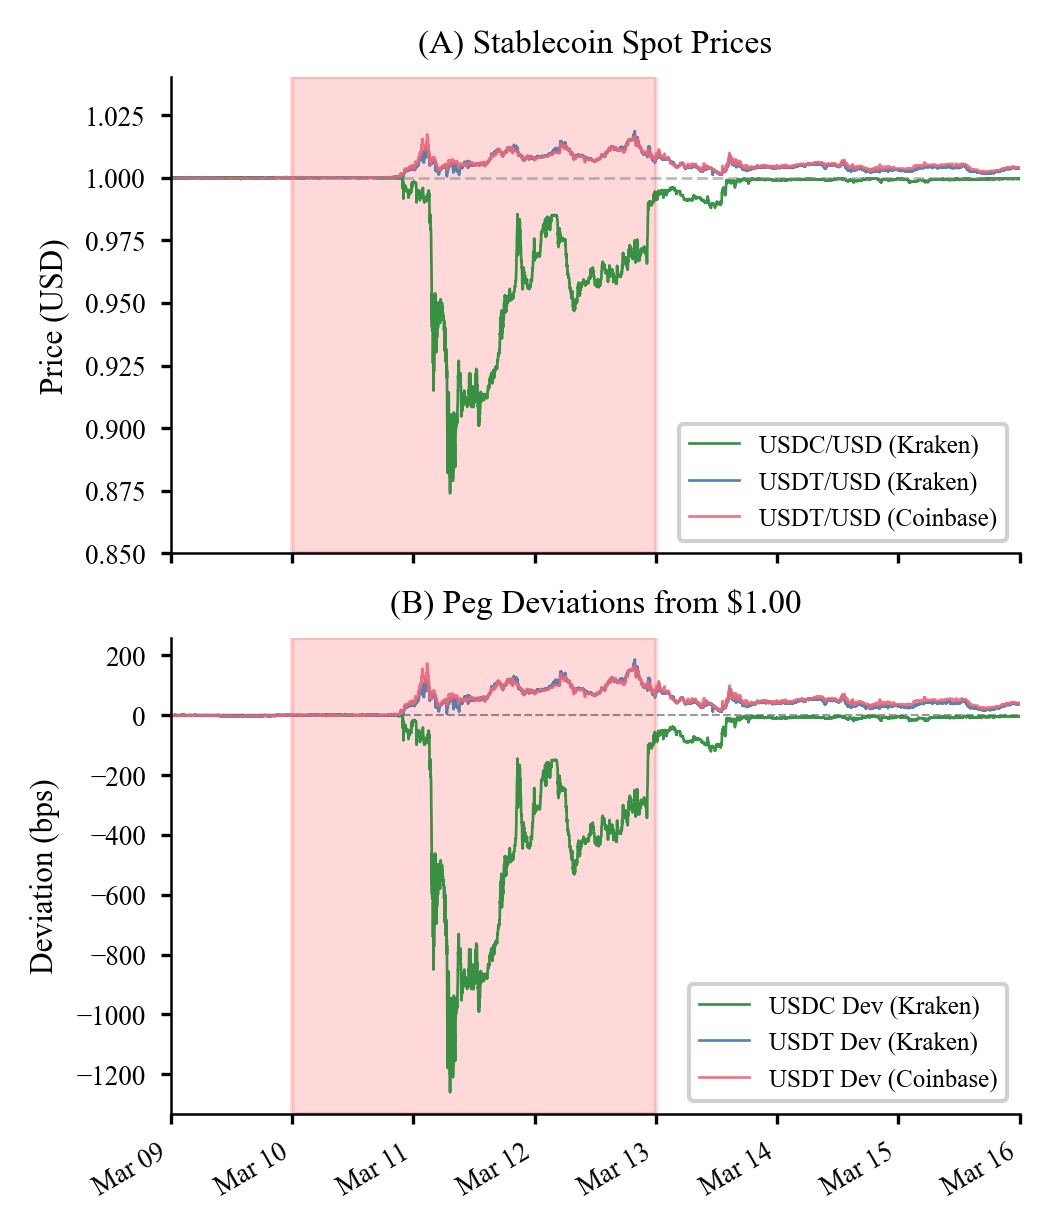
\includegraphics[width=\columnwidth]{figures_col/fig_stablecoin_peg.png}
    \caption{Stablecoin prices (A) and peg deviations (bps, B), March 2023. USDC falls to \$0.874; USDT trades at a premium. Shaded: SVB crisis (March 10--13, UTC).}
    \label{fig:peg}
\end{figure}

We make four contributions. First, we decompose stablecoin-driven fragmentation into a peg-deviation component and an adjusted residual, revealing a ${\sim}940\times$ half-life gap---statistically confirmed via moving-block bootstrap ($p{<}10^{-4}$)---that localizes persistent dislocation to the reserve-access layer. Second, we estimate a contagion intensity model showing that peg stress transmits to the adjusted basis beyond the mechanical price channel ($\hat\lambda$ significant at $p{<}0.001$ during crisis, insignificant pre-SVB), formalizing the two-layer linkage as a testable transmission parameter. Third, we document pronounced asymmetry between USDC and USDT---in tail risk, volatility, contagion direction, and cross-stablecoin correlation---that is inconsistent with a common-shock explanation. Fourth, we map these empirical findings to specific provisions of the GENIUS Act, providing a quantitative lens for evaluating stablecoin regulation.

The remainder of this paper is organized as follows. Section~\ref{sec:data} describes the data and methodology. Section~\ref{sec:results} presents the empirical results across five dimensions: dispersion decomposition, cross-exchange dispersion, market microstructure, price discovery, and arbitrage. Section~\ref{sec:regulation} interprets the findings through a regulatory lens, and Section~\ref{sec:conclusion} concludes.


% ======================================================================
\section{Data and Methodology}\label{sec:data}
% ======================================================================

\subsection{Data sources and preprocessing}
We collect 1-minute OHLCV candles for BTC quoted in USD, USDT, and USDC from Binance (BTC/USDT, BTC/USDC; dominant USDT volume), Coinbase (BTC/USD, BTC/USDT, USDT/USD; primary U.S.\ fiat gateway), and Kraken (BTC/USD, BTC/USDT, BTC/USDC, USDT/USD, USDC/USD; broadest stablecoin-to-fiat coverage). Stablecoin-to-USD conversion uses venue-specific legs. All series are aligned to a 1-minute UTC grid (Table~\ref{tab:data_coverage}). Coverage exceeds 97\% for most series, though pre-SVB Kraken BTC/USDC falls to 89.6\% with 42\% forward-fill share. Short gaps ($\le5$ min) are forward-filled; larger gaps remain NaN. Core directional signs are stable under strict no-FF filtering (crisis USDC $D_t>0$, USDT premium $>0$), though some magnitudes shift on thinner samples. We interpret high-frequency levels as directional unless no-FF retention is adequate.

\begin{table}[H]
\caption{1-minute data coverage and forward-fill exposure on the unified UTC grid. Coverage = non-missing share; FF share = carry-forward share (max 5 minutes).}
\label{tab:data_coverage}
\footnotesize
\resizebox{\columnwidth}{!}{%
\begin{tabular}{lrrrrr}
\toprule
Pair & Coverage Overall (\%) & Coverage Pre-SVB (\%) & Coverage Crisis (\%) & Coverage Post-SVB (\%) & FF Share (\%) \\
\midrule
Kraken BTC/USD   & 99.98  & 100.00 & 100.00 & 99.95  & 0.18  \\
Kraken BTC/USDT  & 98.44  & 97.36  & 99.81  & 99.06  & 30.84 \\
Kraken BTC/USDC  & 94.05  & 89.62  & 99.79  & 96.57  & 42.07 \\
Kraken USDC/USD  & 97.80  & 96.03  & 99.35  & 99.06  & 28.57 \\
Kraken USDT/USD  & 99.98  & 100.00 & 100.00 & 99.95  & 0.91  \\
Coinbase BTC/USD & 99.10  & 97.90  & 100.00 & 100.00 & 0.06  \\
Coinbase BTC/USDT& 98.93  & 97.53  & 99.95  & 99.98  & 17.98 \\
Coinbase USDT/USD& 99.02  & 97.72  & 100.00 & 100.00 & 0.06  \\
Binance BTC/USDT & 100.00 & 100.00 & 100.00 & 100.00 & 0.00  \\
Binance BTC/USDC & 100.00 & 100.00 & 100.00 & 100.00 & 0.00  \\
\bottomrule
\end{tabular}%
}
\end{table}

We proxy transaction frictions using the intra-candle range:
\begin{equation}
    \text{Intra-min Range (bps)} = \left( \frac{\text{High}_t - \text{Low}_t}{\text{Close}_t} \right)\times 10000.
\end{equation}
This is a coarse range proxy that mechanically loads on volatility and microstructure noise; we interpret it cautiously as a friction indicator, not a quoted bid--ask spread.

\subsection{Core quantitative objects}

For stablecoin $Q\in\{\text{USDC}, \text{USDT}\}$, we track two objects. The \emph{unadjusted dispersion}:
\begin{equation}
    D_{Q,t}=\left(\ln(P_{\text{BTC}/Q,t})-\ln(P_{\text{BTC/USD},t})\right)\times 10000,
\end{equation}
and the \emph{adjusted parity residual}:
{\small\begin{equation}
    B_{Q,t}
    = \!\left(\ln(P_{\text{BTC}/Q,t}\!\times\! P_{Q/\text{USD},t})-\ln(P_{\text{BTC/USD},t})\right)\!\times\!10000.
\end{equation}}
These satisfy $B_{Q,t}=D_{Q,t}+10000\cdot\ln(P_{Q/\text{USD},t})$: large de-pegs mechanically drive $D_t$ while $B_t$ captures the residual after marking to USD. Both are computed intra-exchange; cross-venue deviations are studied separately. Basis and dispersion are in log-bps; peg deviations, ranges, and volatility summaries are in arithmetic bps.

\subsection{Mean-reversion dynamics}
We model $B_t$ as an OU process $dX_t = \theta(\mu - X_t)dt + \sigma dW_t$ and estimate the discrete AR(1) form $X_t = c + \rho X_{t-1} + \varepsilon_t$. Stationarity is checked with ADF tests (with large $N$, rejection is expected and serves as a baseline screen). The half-life uses the exact mapping:
\begin{equation}
    \tau_{1/2} = \frac{\ln(2)\,\Delta t}{-\ln(\rho)}, \quad 0<\rho<1.
\end{equation}
If $\rho \le 0$ or $\rho \ge 1$, half-life is undefined (NaN). The OU framework assumes Gaussian innovations; crisis-period $B_t$ exhibits substantial excess kurtosis (Section~\ref{sec:liq_vol}), so we use the AR(1) model solely for its half-life mapping, not as a full distributional model. We report robustness at 5-minute sampling and with forward-filled minutes removed.

\subsection{Contagion intensity model}\label{sec:contagion_model}
The univariate OU model treats the adjusted basis $B_t$ in isolation from the peg layer. To formalize the inter-layer linkage, we extend the mean-reversion equation to include lagged peg deviation $S_t$ (in bps) as a forcing variable:
\begin{equation}\label{eq:contagion}
    \Delta B_t = a + \beta\, B_{t-1} + \lambda\, S_{t-1} + \varepsilon_t,
\end{equation}
where the \emph{contagion intensity} $\lambda$ measures the marginal rate at which peg-layer stress transmits to the cross-currency basis after stablecoin-to-USD adjustment. When peg risk is fully absorbed by the conversion leg, $\lambda{=}0$ and $B_t$ follows a standard AR(1). Rejection of $\lambda{=}0$ indicates residual transmission---via liquidity withdrawal, adverse selection, or order-book asymmetry---beyond the mechanical price channel. We estimate~(\ref{eq:contagion}) by OLS with HAC standard errors (Newey--West, 60 lags) \cite{neweywest1987} separately for each regime, so that both the mean-reversion speed $\hat\rho{=}1{+}\hat\beta$ and the contagion parameter $\hat\lambda$ are regime-specific. The lagged structure avoids simultaneity: reverse causation from $B_t$ to the peg price is implausible at the 1-minute horizon because arbitrageurs correcting $B_t$ do not move the aggregate stablecoin/USD rate.

\subsection{Price discovery framework}
For the two primary Kraken channels (BTC/USD vs.\ BTC/USDC and BTC/USD vs.\ BTC/USDT), we use synchronized 1-minute log-price levels, dropping forward-filled minutes. We test for cointegration with Johansen trace tests (constant restricted to the cointegration relation; lag order via BIC on the levels VAR) \cite{johansen1988,englegranger1987}. When rank $=1$, we estimate:
\begin{equation}
    \Delta \mathbf{p}_t = \alpha \beta^\top \mathbf{p}_{t-1} + \sum_{i=1}^{k_{\Delta}} \Gamma_i \Delta \mathbf{p}_{t-i} + \mathbf{u}_t.
\end{equation}
The market with smaller $|\alpha|$ adjusts less and is interpreted as the relative leader. We retain BH/FDR-corrected Granger tests on returns as secondary evidence only \cite{granger1969}; with 1-minute bars, asynchrony and large $N$ can overstate economic lead--lag strength.

% ======================================================================
\section{Empirical Results}\label{sec:results}
% ======================================================================

\subsection{Dispersion, adjusted residual, and mean reversion}

\begin{figure}[H]
    \centering
    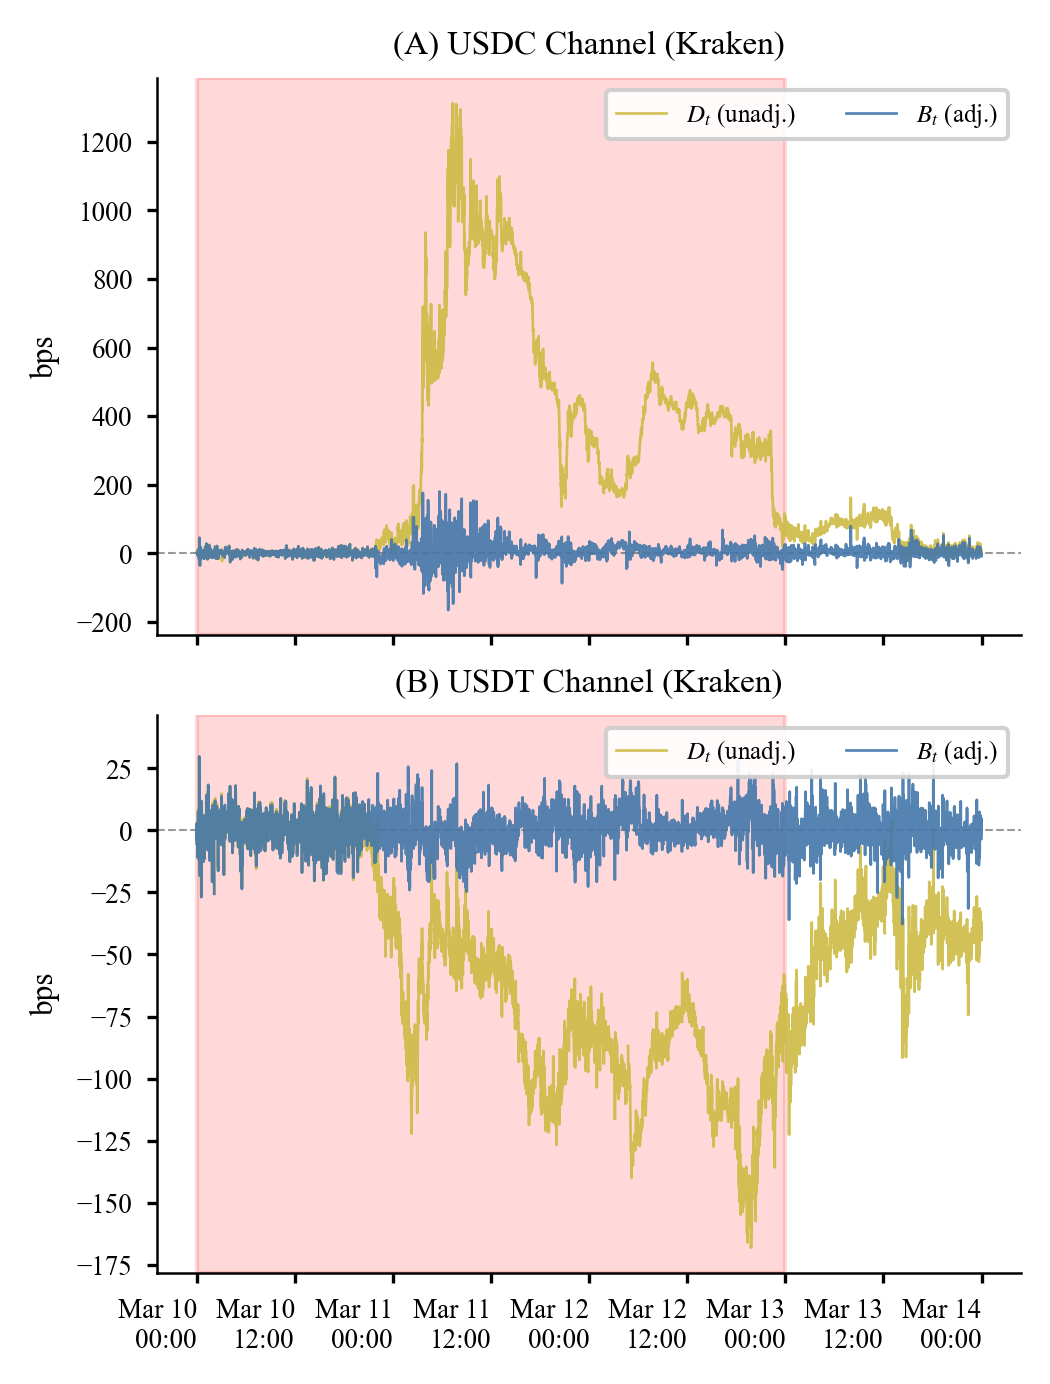
\includegraphics[width=\columnwidth]{figures_col/fig_dispersion_vs_adjusted_kraken.png}
    \caption{Kraken crisis decomposition: unadjusted dispersion $D_t$ vs.\ adjusted residual $B_t$. USDC $D_t$ exceeds $+1{,}200$ bps while $B_t$ stays within $\pm150$ bps; for USDT, $D_t$ reflects the premium and $B_t\approx0$.}
    \label{fig:decomp}
\end{figure}

Before SVB, both $D_t$ and $B_t$ hover near zero. During the crisis (March 10--13 UTC), USDC dispersion jumps to $+320$ bps ($\sigma{=}323$) while the adjusted residual remains small ($+5.3$ bps, $\sigma{=}21$). USDT moves oppositely: $D_t{=}{-}57$ bps, $B_t{=}{+}0.7$ bps (Table~\ref{tab:dispersion_vs_adjusted}). Figure~\ref{fig:decomp} visualizes this: $D_t$ (orange) captures the peg shift while $B_t$ (blue) remains tightly mean-reverting.

Two dynamics drive this pattern. USDC trades as low as \$0.874 on Kraken on March 11 (${\approx}{-}1{,}260$ bps), mechanically pulling $D_t$ upward; simultaneously, USDT trades at a premium averaging $+58.1$ bps on Kraken and $+59.7$ on Coinbase. Figure~\ref{fig:substitution} visualizes this stablecoin substitution: crisis observations (red) migrate to the lower-right quadrant ($D_{\text{USDC}}>0$, $D_{\text{USDT}}<0$), and the unadjusted cross-stablecoin correlation flips from $+0.44$ to $-0.42$---consistent with traders rotating out of USDC into USDT under stress.

% Single-column figure (portrait scatter -- fits in one column)
\begin{figure}[H]
    \centering
    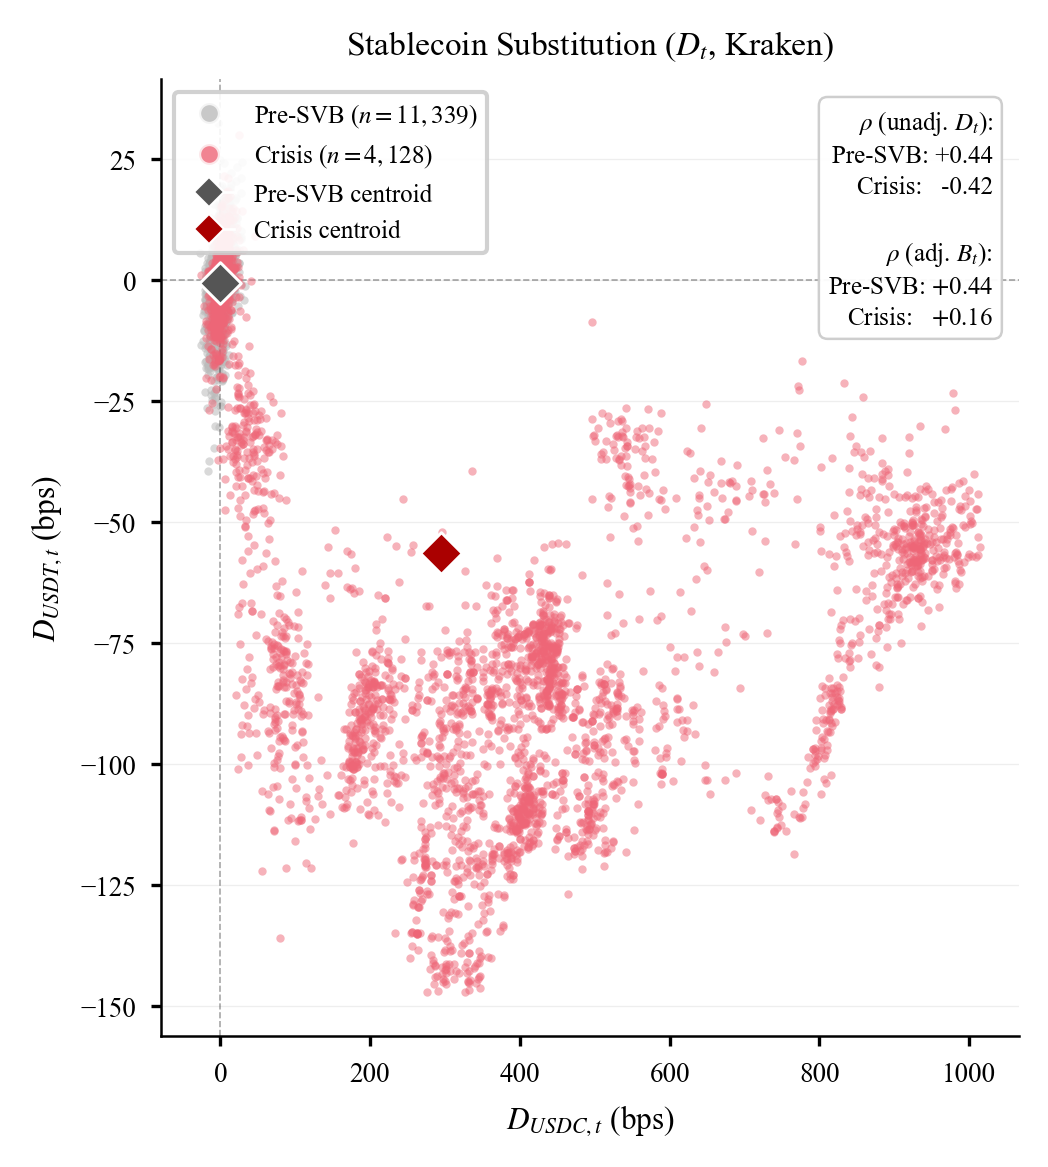
\includegraphics[width=\columnwidth]{figures_col/fig_stablecoin_substitution_scatter.png}
    \caption{Kraken stablecoin substitution: $D_{\text{USDC},t}$ vs.\ $D_{\text{USDT},t}$. Crisis points shift to the lower-right quadrant; unadjusted correlation flips ($+0.44\to-0.42$) and adjusted $B_t$ correlation falls ($0.44\to0.16$).}
    \label{fig:substitution}
\end{figure}

\begin{table}[H]
\caption{Kraken regime statistics for unadjusted dispersion ($D_t$) and adjusted residual ($B_t$), in bps.}
\label{tab:dispersion_vs_adjusted}
\footnotesize
\resizebox{\columnwidth}{!}{%
\begin{tabular}{llrrrr}
\toprule
Regime & Series & Mean (bps) & Std (bps) & Mean Abs (bps) & N \\
\midrule
Pre-SVB  & USDC $D_t$ (Unadj.) &    0.12 &   4.95 &   3.49 & 11615 \\
Pre-SVB  & USDC $B_t$ (Adj.)   &   -0.32 &   5.00 &   3.53 & 11197 \\
Pre-SVB  & USDT $D_t$ (Unadj.) &   -0.54 &   4.49 &   3.17 & 12618 \\
Pre-SVB  & USDT $B_t$ (Adj.)   &   -0.60 &   4.33 &   3.02 & 12618 \\
Crisis   & USDC $D_t$ (Unadj.) &  319.97 & 322.87 & 321.17 &  4311 \\
Crisis   & USDC $B_t$ (Adj.)   &    5.27 &  21.21 &  13.37 &  4283 \\
Crisis   & USDT $D_t$ (Unadj.) &  -57.18 &  45.10 &  58.57 &  4312 \\
Crisis   & USDT $B_t$ (Adj.)   &    0.68 &   6.57 &   4.94 &  4312 \\
Post-SVB & USDC $D_t$ (Unadj.) &   11.22 &  21.95 &  14.27 & 12514 \\
Post-SVB & USDC $B_t$ (Adj.)   &    0.45 &   9.06 &   6.68 & 12419 \\
Post-SVB & USDT $D_t$ (Unadj.) &  -30.26 &  13.29 &  30.28 & 12837 \\
Post-SVB & USDT $B_t$ (Adj.)   &   -1.23 &   6.47 &   4.92 & 12837 \\
\bottomrule
\end{tabular}%
}
\end{table}

HAC/Newey--West intervals (60-lag cap) confirm directional robustness \cite{neweywest1987}: USDC crisis $D_t$ 95\% CI $[245.7,\,394.3]$ bps; crisis $B_t$ CI $[3.6,\,7.0]$ bps; USDT premiums positive on both Kraken ($[47.4,\,68.8]$) and Coinbase ($[49.1,\,70.3]$). Coinbase--Kraken BTC/USD remains significantly positive ($[1.7,\,2.6]$ bps).

ADF rejects a unit root for all $B_t$ channels ($p<0.001$). Kraken USDC half-life: $0.98$ min pre-SVB, $0.61$ min crisis, $0.79$ min post-SVB. Figure~\ref{fig:halflife_robust} shows robustness across 1m/5m sampling and all/no-FF filters: USDC crisis half-life ranges from $0.54$ to $1.10$ min; USDT crisis half-life is longer ($0.92$--$3.06$ min). Fast USDC mean reversion is robust across all specifications.

% Full-width figure (dot-plot across regimes/specs)
\begin{figure}[H]
    \centering
    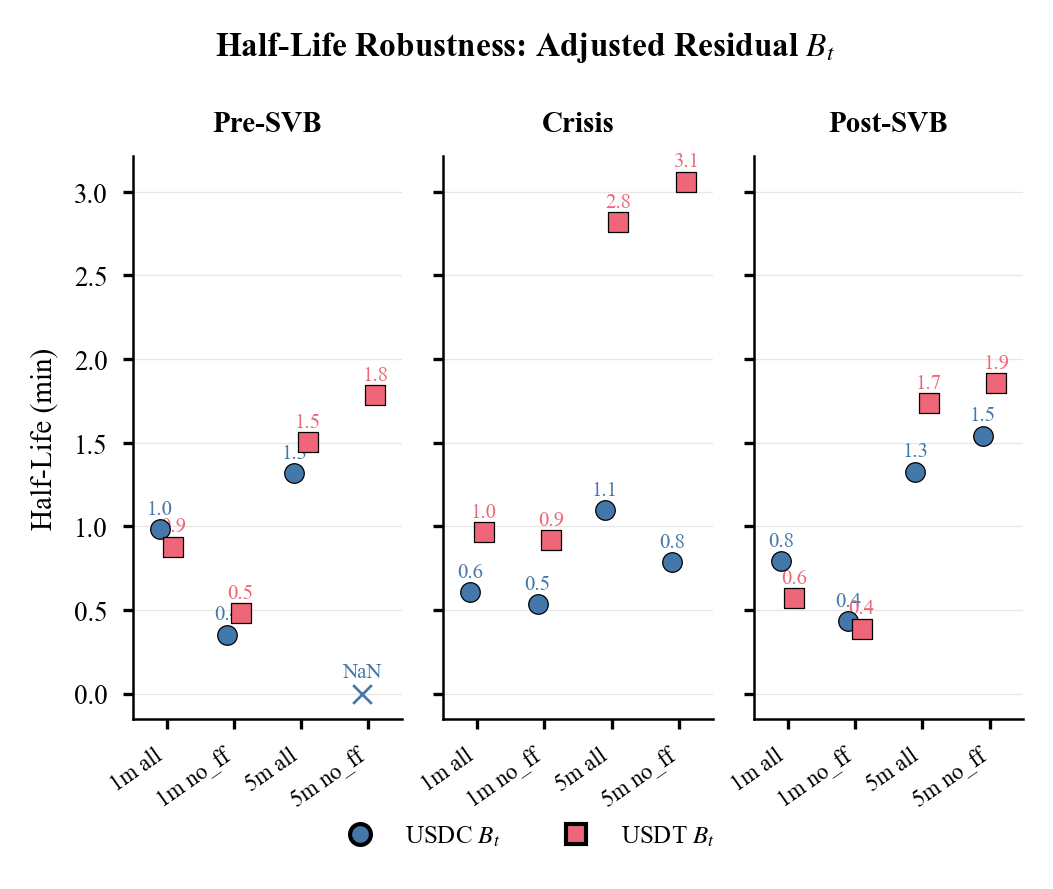
\includegraphics[width=\columnwidth]{figures_col/fig_half_life_robustness.png}
    \caption{Adjusted-residual $B_t$ half-life robustness by regime/specification (1m/5m $\times$ all/no-FF). USDC crisis half-life stays below 1.1 min; USDT reaches 3.1 min (5m no-FF).}
    \label{fig:halflife_robust}
\end{figure}

\begin{figure}[H]
    \centering
    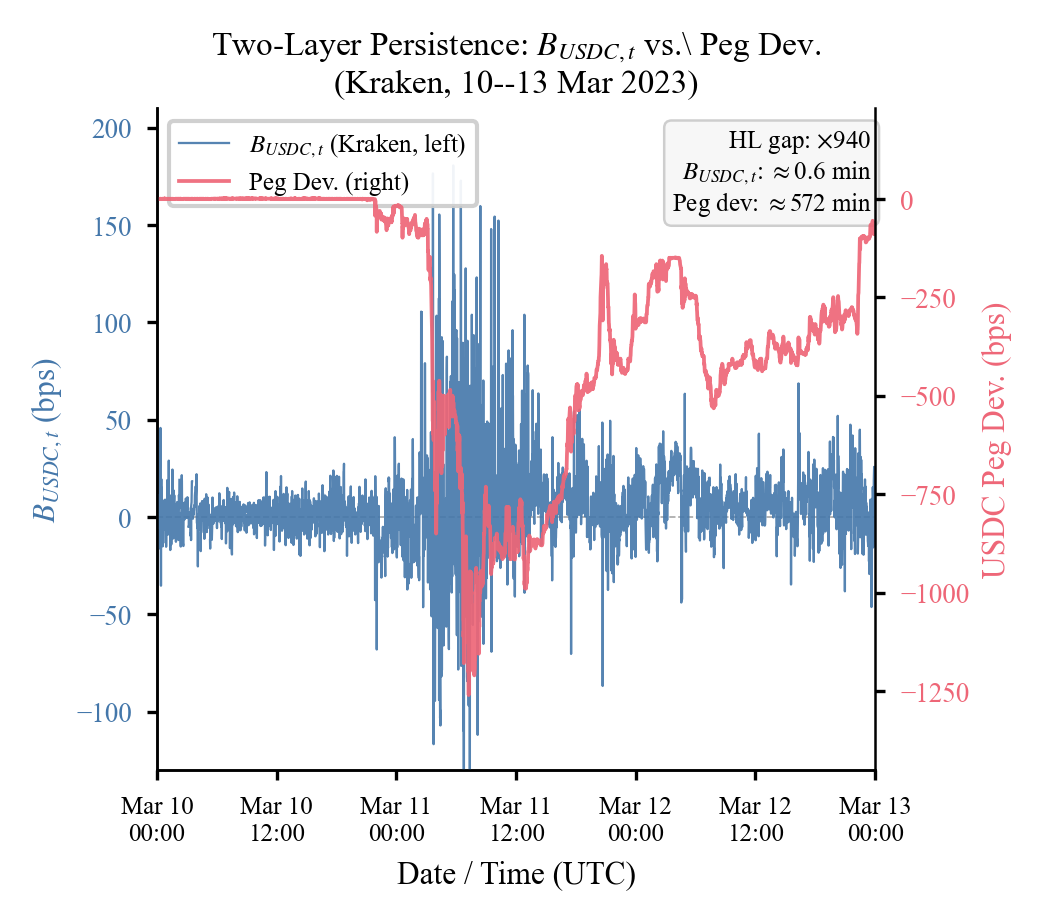
\includegraphics[width=\columnwidth]{figures_col/fig_two_layer_persistence.png}
    \caption{Two-layer persistence (March 10--13): $B_{\text{USDC},t}$ mean-reverts in ${\approx}0.6$ min, while the USDC peg deviation persists for ${\approx}572$ min. The ${\sim}940\times$ gap localizes persistent dislocation to the peg layer.}
    \label{fig:twolayer}
\end{figure}

The OU estimation reveals a \textbf{two-layer dynamic} (Figure~\ref{fig:twolayer}): $B_t$ mean-reverts in ${\approx}0.6$ min during crisis ($\hat\rho{=}0.320$), while the USDC peg deviation persists with half-life ${\approx}572$ min ($\hat\rho{=}0.999$, ADF $p{=}0.44$); USDT peg deviations similarly persist ($496$--$542$ min). The point-estimate ratio $R{=}\tau_{1/2}^{\text{peg}}/\tau_{1/2}^{B}{\approx}940$ is striking, but could in principle reflect estimation noise. A moving-block bootstrap (5{,}000 replications; block length 60 minutes) yields $R_{\text{median}}{=}567$ with 95\% CI $[216,\,1{,}898]$ and $p{<}10^{-4}$ for $H_0{:}\;R{\le}1$. The persistence gap is statistically overwhelming: cross-market correction is fast even in crisis, but the peg itself---driven by reserve-access risk---is where dislocation persists.

\paragraph{Contagion intensity.}
Whether the two layers interact beyond the mechanical decomposition identity is an empirical question. Estimating the coupled model~(\ref{eq:contagion}), we find that the contagion intensity $\hat\lambda$ is indistinguishable from zero pre-SVB ($-0.002$, $p{=}0.98$) but becomes significantly negative during the crisis ($-0.009$, $p{<}0.001$) and remains elevated post-SVB ($-0.019$, $p{=}0.006$); see Table~\ref{tab:contagion}. Because $S_t{<}0$ corresponds to a peg discount (USDC below par), the negative $\hat\lambda$ implies that a deeper peg discount at $t{-}1$ pushes $B_t$ upward at $t$---consistent with liquidity withdrawal from the USDC book creating transient positive residual basis even after marking to USD. USDT displays the mirror pattern: $\hat\lambda{=}{+}0.019$ during crisis ($p{<}0.001$), so a USDT premium at $t{-}1$ pulls $B_t$ upward---consistent with safe-haven demand spilling into the adjusted residual. These sign patterns confirm that peg stress does not merely drive $D_t$ mechanically but also transmits to $B_t$ through microstructure channels, and that the two stablecoins propagate stress in opposite directions.

\begin{table}[H]
\caption{Contagion intensity $\hat\lambda$ from Eq.~(\ref{eq:contagion}): regime-specific OLS with Newey--West HAC (60 lags). $S_t$ is the peg deviation (bps; negative = discount).}
\label{tab:contagion}
\footnotesize
\centering
\resizebox{\columnwidth}{!}{%
\begin{tabular}{llrrrrrr}
\toprule
Channel & Regime & $\hat\lambda$ & SE & $t$-stat & $p$-value & $R^2$ & $N$ \\
\midrule
USDC & Pre-SVB  & $-$0.002 & 0.091 & $-$0.02 & 0.985 & 0.253 & 11{,}196 \\
USDC & Crisis   & $-$0.009 & 0.002 & $-$4.77 & ${<}0.001$ & 0.351 & 4{,}282 \\
USDC & Post-SVB & $-$0.019 & 0.007 & $-$2.73 & 0.006 & 0.293 & 12{,}418 \\
\midrule
USDT & Pre-SVB  & $-$0.076 & 0.032 & $-$2.38 & 0.017 & 0.273 & 12{,}617 \\
USDT & Crisis   & $+$0.019 & 0.004 & $+$5.23 & ${<}0.001$ & 0.272 & 4{,}311 \\
USDT & Post-SVB & $+$0.023 & 0.008 & $+$2.80 & 0.005 & 0.354 & 12{,}836 \\
\bottomrule
\end{tabular}%
}
\end{table}

Robustness is strong: the USDC crisis $\hat\lambda$ is significant under no-forward-fill sampling ($-0.009$, $p{<}0.001$, $N{=}3{,}001$) and at 5-minute frequency ($-0.012$, $p{<}0.001$, $N{=}861$). For USDT, the sign flip between pre-SVB ($\hat\lambda{<}0$) and crisis ($\hat\lambda{>}0$) coincides precisely with the shift from normal co-movement to safe-haven dynamics, consistent with the correlation break documented below.

Figure~\ref{fig:crisiszoom} provides a granular minute-by-minute view of all channels during the peak crisis window. Panel~A reveals that the USDC adjusted residual (green) exhibits extreme volatility---spikes exceeding $+150$ bps---while the USDT channels on both Kraken and Coinbase remain tightly bounded near zero. Panel~B shows that cross-exchange differentials widen simultaneously, with the Coinbase--Kraken BTC/USD basis rising to $+60$ bps, suggesting stress propagation across venues.

\begin{figure}[H]
    \centering
    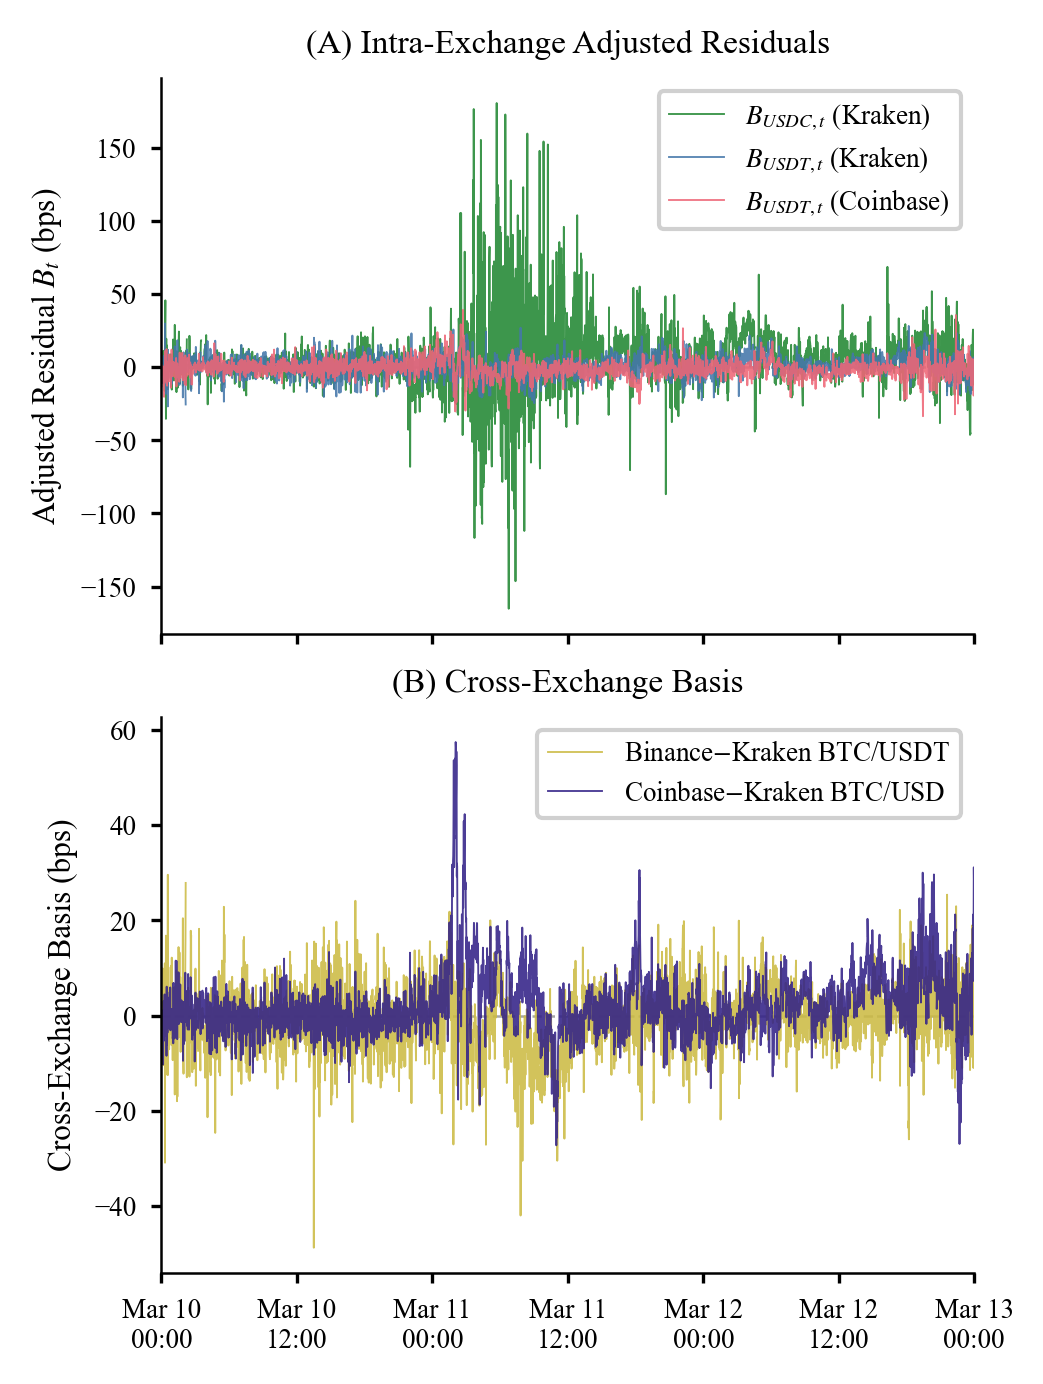
\includegraphics[width=\columnwidth]{figures_col/fig_svb_crisis_zoom.png}
    \caption{Crisis zoom (March 10--13). (A)~$B_{\text{USDC},t}$ spikes past $\pm150$ bps while USDT stays within $\pm30$ bps. (B)~Cross-exchange basis widens simultaneously, indicating stress propagation across venues.}
    \label{fig:crisiszoom}
\end{figure}

\subsection{Cross-exchange price dispersion}

\begin{figure}[H]
    \centering
    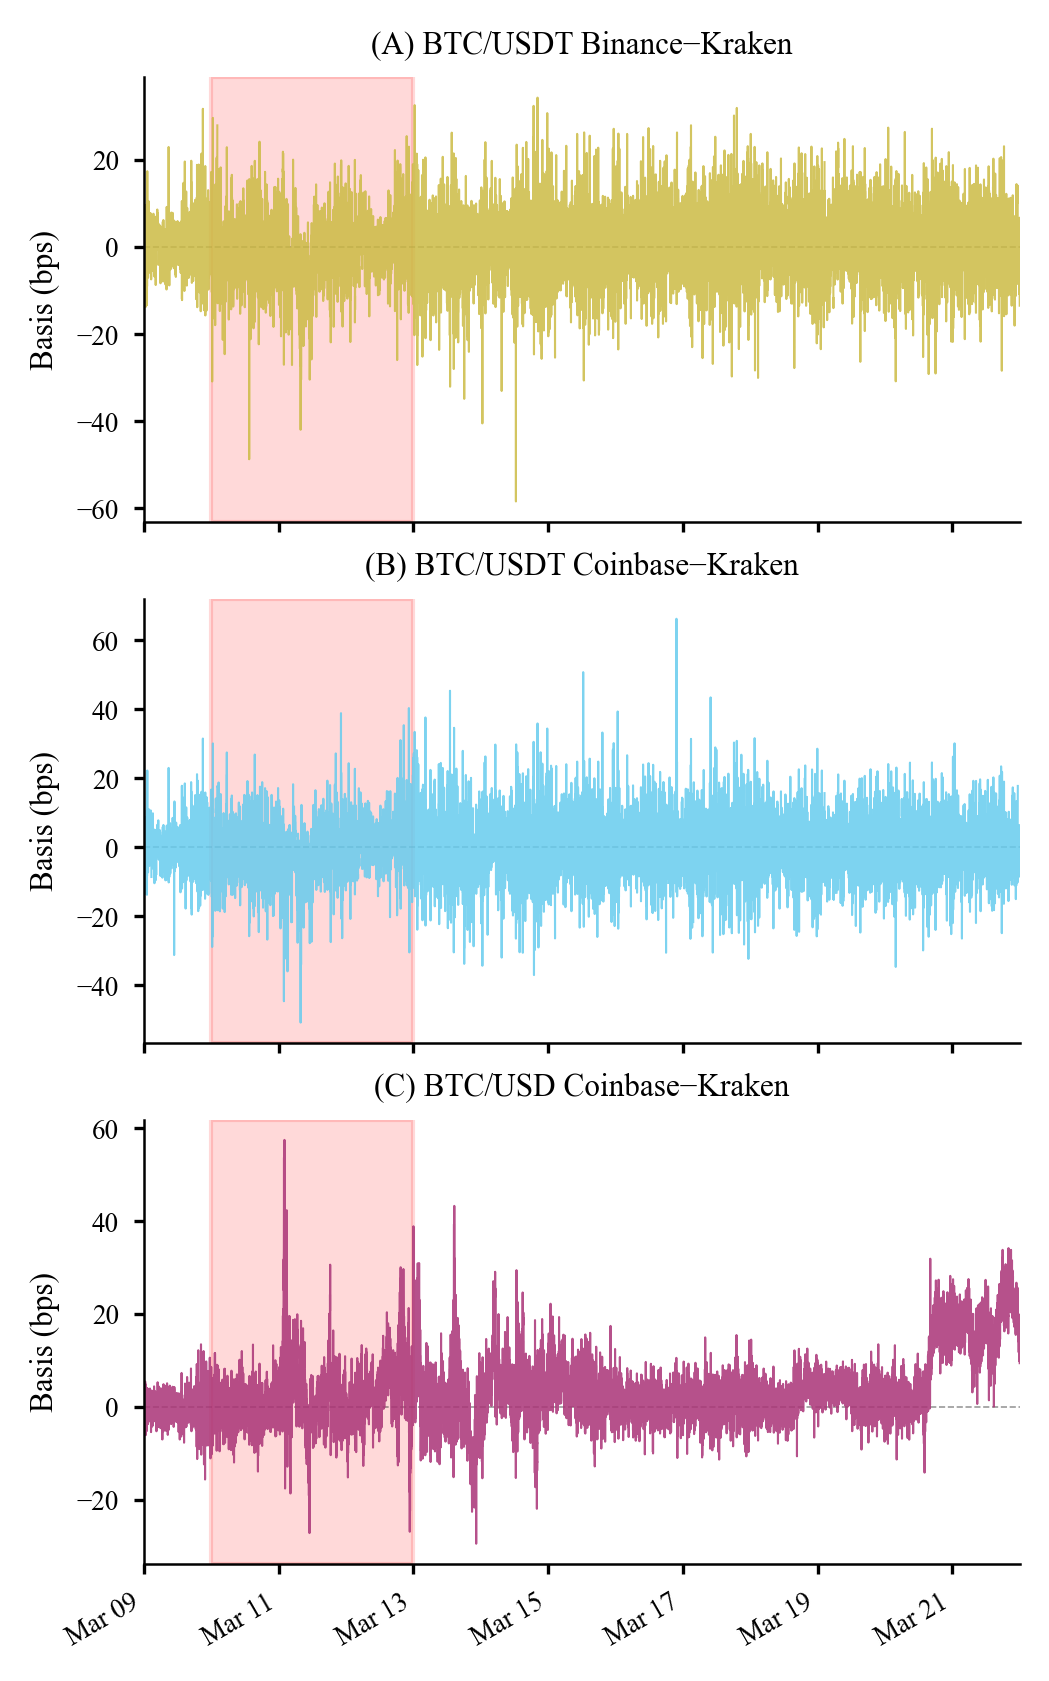
\includegraphics[width=\columnwidth]{figures_col/fig_cross_exchange_basis.png}
    \caption{Cross-exchange basis (bps): BTC/USDT Binance--Kraken (A), Coinbase--Kraken (B), and BTC/USD Coinbase--Kraken (C). The fiat channel stays persistently positive and elevated post-crisis.}
    \label{fig:xbasis}
\end{figure}

Having established that intra-exchange fragmentation is dominated by USDC peg risk, a natural question is whether this dislocation propagates \emph{across} exchanges. We examine this by computing log-price differentials for BTC/USDT (Binance vs.\ Kraken; Coinbase vs.\ Kraken) and BTC/USD (Coinbase vs.\ Kraken). Caveat: USDT cross-exchange dispersion is in the USDT numeraire; a USD-based arbitrage requires an additional USDT/USD leg. Binance--Kraken BTC/USDT is near zero full-sample ($+0.007$ bps), consistent with tight integration. Coinbase--Kraken BTC/USD shows a persistent $+2.18$ bps premium, consistent with a structural U.S.\ fiat gateway effect.

During the crisis, cross-exchange differentials widen alongside intra-exchange deviations (Figure~\ref{fig:xbasis}, Table~\ref{tab:arb}), consistent with broad stress rather than a single-venue disruption. The Coinbase--Kraken fiat premium did not fully normalize post-crisis, suggesting it partly reflects structural microstructure differences that stress amplified.

\subsection{Market microstructure dynamics}\label{sec:liq_vol}
The cross-exchange widening documented above raises the question of whether liquidity conditions differ materially across channels. We quantify liquidity with the Roll (1984) effective spread \cite{roll1984} and Amihud (2002) ILLIQ ratio \cite{amihud2002}. Table~\ref{tab:liquidity_spread} and Figure~\ref{fig:liq} report regime means. Kraken BTC/USDC Roll spread jumps $23\times$ ($1.10$ to $25.64$ bps), while BTC/USDT holds near $3$ bps. Amihud confirms Coinbase BTC/USD is deepest and Kraken BTC/USDC least liquid. The two measures diverge in crisis: Roll widens while Amihud declines as volume surges.

% Full-width figure (two panels)
\begin{figure}[H]
    \centering
    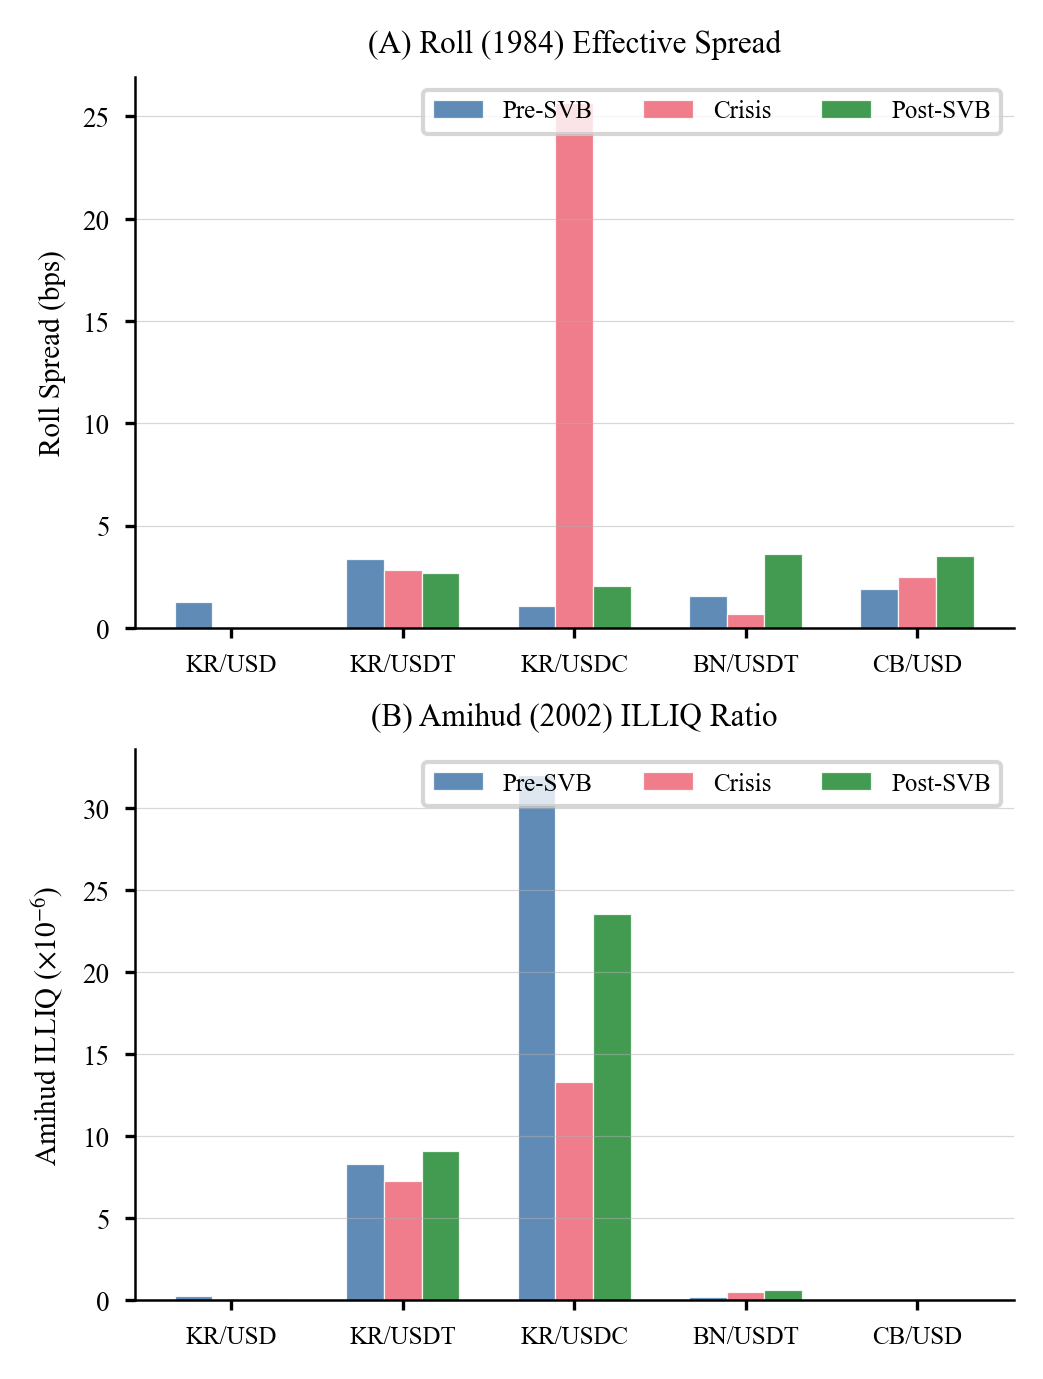
\includegraphics[width=\columnwidth]{figures_col/fig_liquidity_roll_amihud.png}
    \caption{Roll effective spread (A) and Amihud ILLIQ (B) by pair/regime. Kraken BTC/USDC shows a $23\times$ Roll spread blowout in crisis. Roll is undefined when serial covariance is non-negative; thin-pair means are indicative.}
    \label{fig:liq}
\end{figure}

\begin{table}[H]
\caption{Roll effective spread (bps) and Amihud illiquidity ($\times10^{-6}$) by pair/regime. Roll uses daily serial covariance of 1-minute log returns (NaN days excluded; $N$ = valid Roll days). ILLIQ$_t = |r_t|/\text{DollarVol}_t$ (daily average).}
\label{tab:liquidity_spread}
\footnotesize
\resizebox{\columnwidth}{!}{%
\begin{tabular}{lrrrrrrrrr}
\toprule
Pair & Roll\textsubscript{Pre} & Roll\textsubscript{Crisis} & Roll\textsubscript{Post} & $N$\textsubscript{Pre} & $N$\textsubscript{Crisis} & $N$\textsubscript{Post} & ILLIQ\textsubscript{Pre} & ILLIQ\textsubscript{Crisis} & ILLIQ\textsubscript{Post} \\
\midrule
Kraken BTC/USD  & 1.260 & ---    & ---   & 4 & 0 & 0 & 0.232  & 0.050  & 0.068  \\
Kraken BTC/USDT & 3.390 & 2.850  & 2.670 & 1 & 1 & 1 & 8.299  & 7.266  & 9.074  \\
Kraken BTC/USDC & 1.100 & 25.640 & 2.070 & 2 & 2 & 2 & 31.970 & 13.282 & 23.530 \\
Binance BTC/USDT& 1.560 & 0.670  & 3.630 & 6 & 1 & 5 & 0.163  & 0.461  & 0.591  \\
Coinbase BTC/USD& 1.880 & 2.490  & 3.490 & 5 & 1 & 1 & 0.005  & 0.003  & 0.003  \\
\bottomrule
\end{tabular}%
}
\end{table}

Daily dollar-volume depth proxies (Table~\ref{tab:depth_proxy}) sharpen this picture: Coinbase BTC/USD is the deepest channel (\$239M pre-SVB, rising to \$664M post-SVB), while Kraken BTC/USDC is $26\times$ thinner in crisis (\$15.7M vs.\ \$407M). The depth gap constrains the scale at which arbitrageurs can trade the USDC dislocation, consistent with the limited post-friction profitability documented in Section~\ref{sec:arb}.

\begin{table}[H]
\caption{Daily traded dollar volume by pair/regime (median, \$MM/day). Dollar volume serves as a depth proxy where L2 order-book data is unavailable.}
\label{tab:depth_proxy}
\footnotesize
\resizebox{\columnwidth}{!}{%
\begin{tabular}{lrrr}
\toprule
Pair & Pre-SVB & Crisis & Post-SVB \\
\midrule
Kraken BTC/USD   & 59.50  & 160.36 & 203.77 \\
Kraken BTC/USDT  &  5.55  &  13.84 &  17.37 \\
Kraken BTC/USDC  &  2.56  &  15.65 &   5.52 \\
Binance BTC/USDT & 52.44  &  73.92 &  71.46 \\
Coinbase BTC/USD & 239.07 & 407.27 & 664.46 \\
\bottomrule
\end{tabular}%
}
\end{table}

HAC regressions (Newey--West, 60 lags) of $B_t$ on a crisis dummy, realized volatility, and range proxy (Table~\ref{tab:regression_hac}) show a significant USDC crisis coefficient ($+4.30$ bps, $p<0.001$) \cite{neweywest1987}. Explanatory power is modest ($R^2=0.041$), so we interpret these as partial associations.

\begin{table}[H]
\caption{HAC regressions of Kraken adjusted residual $B_t$ on crisis, realized volatility, and range proxy (Newey--West, 60 lags).}
\label{tab:regression_hac}
\footnotesize
\centering
\resizebox{\columnwidth}{!}{%
\begin{tabular}{lcccc}
\toprule
 & \multicolumn{2}{c}{USDC Channel} & \multicolumn{2}{c}{USDT Channel} \\
\cmidrule(lr){2-3} \cmidrule(lr){4-5}
 & Coef. & $p$-value & Coef. & $p$-value \\
\midrule
Constant          & $-0.079$ & 0.833   & $-0.656$ & $<0.001$ \\
Crisis            & $+4.295$ & $<0.001$& $+1.655$ & $<0.001$ \\
RealizedVol (60m) & $+0.004$ & 0.928   & $-0.029$ & 0.179    \\
Range Proxy       & $+0.048$ & 0.005   & $-0.013$ & 0.082    \\
\midrule
$R^2$             & \multicolumn{2}{c}{0.041}  & \multicolumn{2}{c}{0.012}  \\
$N$               & \multicolumn{2}{c}{26,489} & \multicolumn{2}{c}{26,489} \\
\bottomrule
\multicolumn{5}{l}{\footnotesize OLS with HAC standard errors (Newey--West, 60 lags). Dependent variable: $B_t$ (bps).}
\end{tabular}%
}
\end{table}

Figure~\ref{fig:volshare} shows daily volume fragmentation: USDC share doubles during crisis (2.1\% to 4.3\%) as activity concentrates in Kraken BTC/USDC, while post-crisis USD dominance returns (86.9\%).

% Full-width figure
\begin{figure}[H]
    \centering
    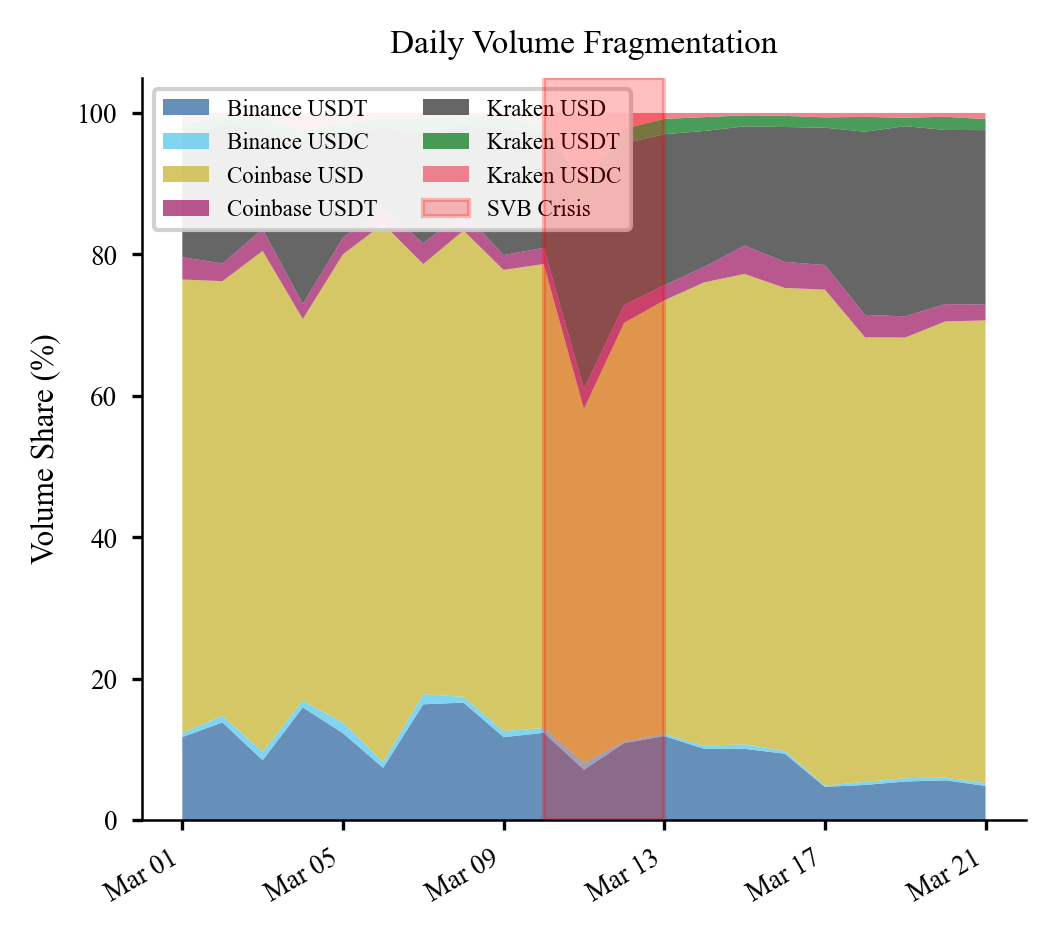
\includegraphics[width=\columnwidth]{figures_col/fig_volume_share.png}
    \caption{Daily volume shares across pairs. USDC share spikes during the crisis (Kraken BTC/USDC surge) and rotates back to USD post-crisis.}
    \label{fig:volshare}
\end{figure}

Realized volatility (Figure~\ref{fig:realvol}) reveals pronounced asymmetry: Kraken BTC/USDC peaks at ${\approx}650$ bps/hr on March 11, roughly $2.1\times$ the crisis-average for BTC/USD and BTC/USDT---consistent with compounding asset risk and numeraire risk.

% Full-width figure
\begin{figure}[H]
    \centering
    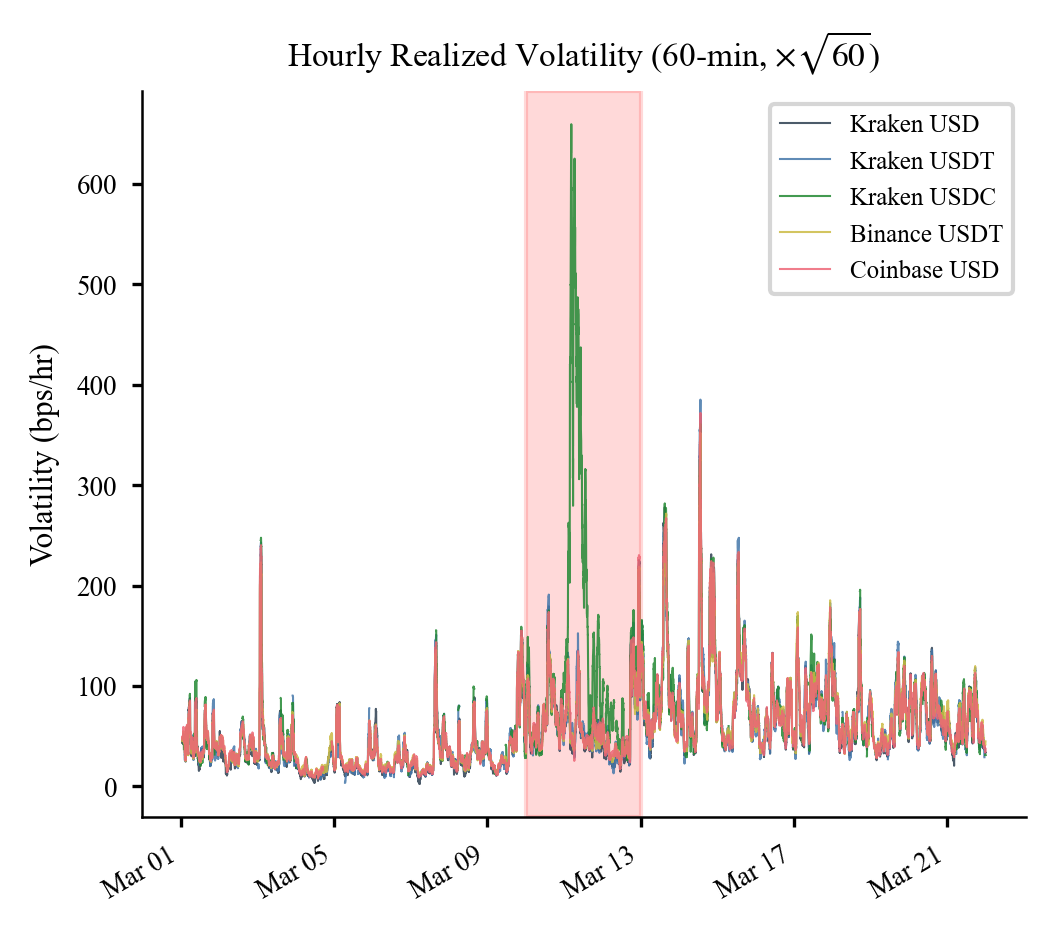
\includegraphics[width=\columnwidth]{figures_col/fig_realized_volatility.png}
    \caption{Hourly realized volatility (60-min rolling $\sigma$, $\times\sqrt{60}$) by pair. Kraken BTC/USDC peaks near ${\approx}650$ bps/hr in crisis, about $2.1\times$ the USD and USDT channels.}
    \label{fig:realvol}
\end{figure}

\begin{figure}[H]
    \centering
    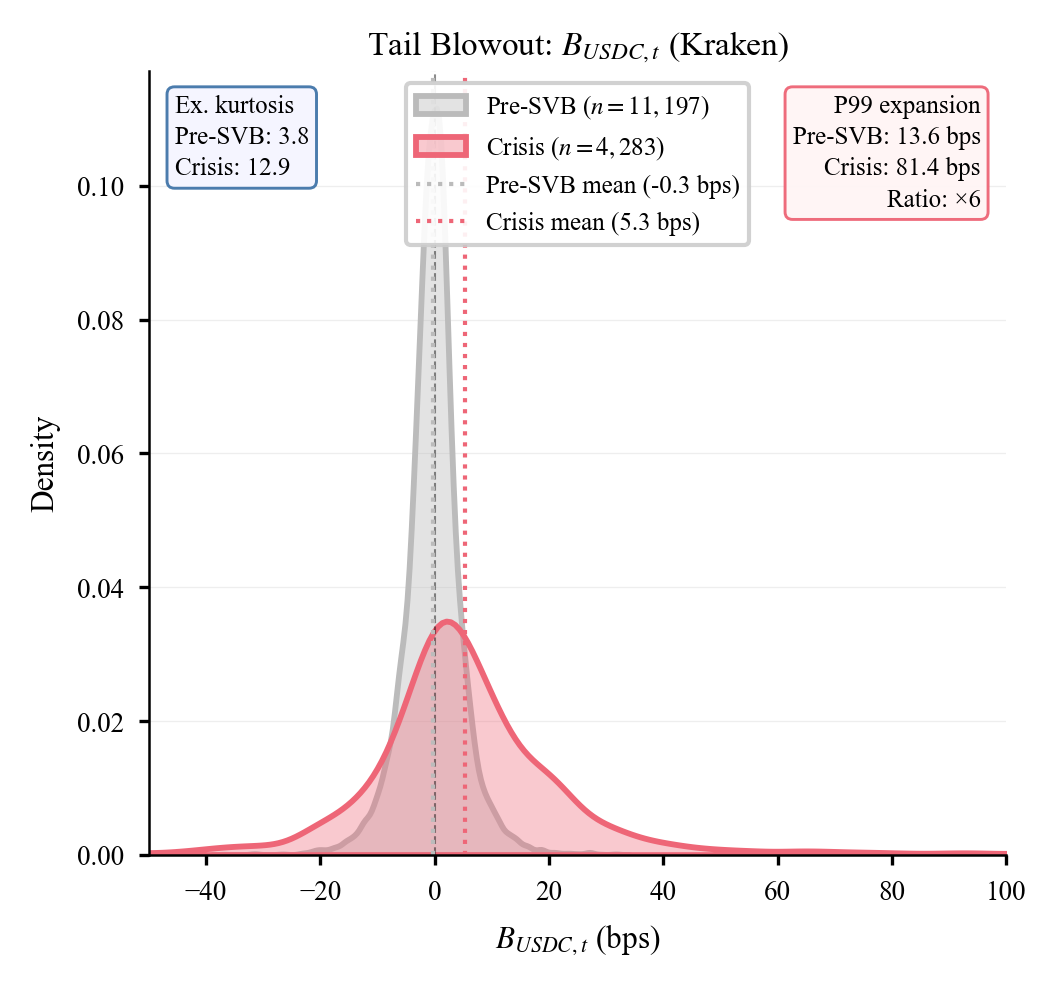
\includegraphics[width=\columnwidth]{figures_col/fig_tail_blowout_kde.png}
    \caption{Kraken distribution of USDC adjusted residual $B_{\text{USDC},t}$: pre-SVB vs.\ crisis. Crisis shows a right shift, excess kurtosis 12.9 (vs.\ 3.8), and a $6\times$ increase in the 99th percentile (13.6 to 81.4 bps).}
    \label{fig:tailblowout}
\end{figure}

The distributional impact is stark (Figure~\ref{fig:tailblowout}): crisis USDC $B_t$ develops tails beyond $\pm100$ bps versus $\pm10$ bps pre-SVB. For risk management, stablecoin positions carry latent peg-break tail risk that calm-calibrated VaR models materially understate.

% Single-column figure (portrait KDE -- fits in one column)

\paragraph{Distributional robustness.}

\begin{figure}[H]
    \centering
    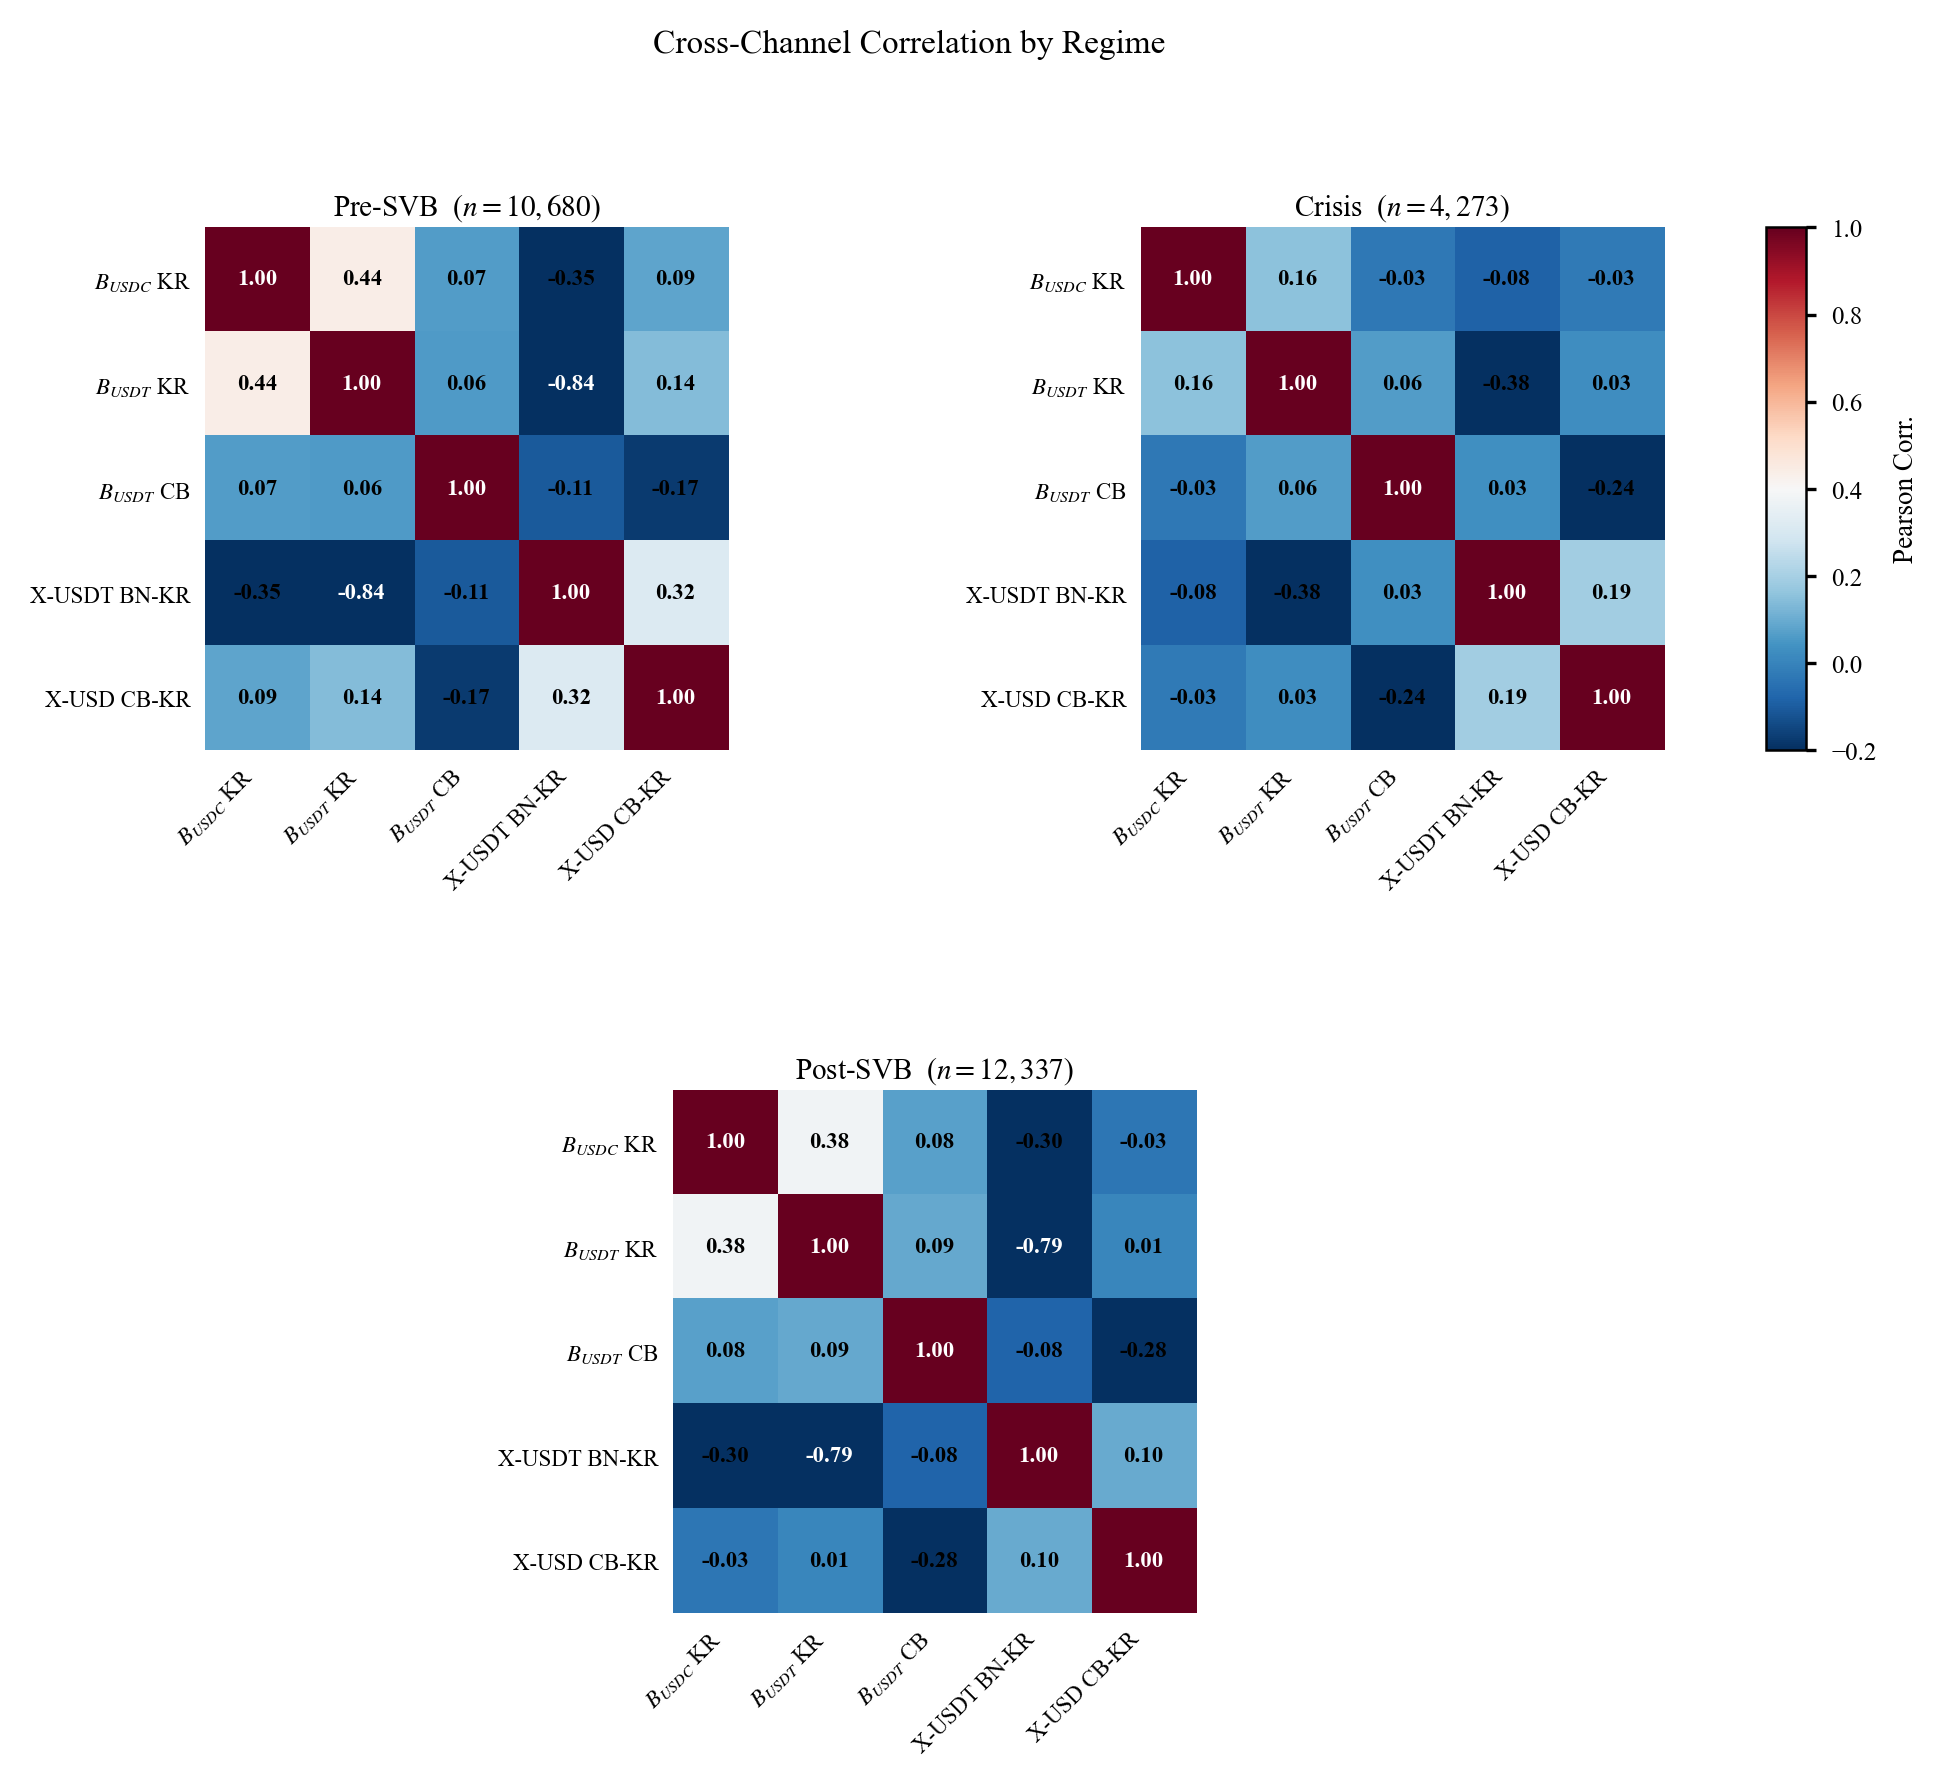
\includegraphics[width=\columnwidth]{figures_col/fig_correlation_regime_heatmap.png}
    \caption{Regime correlation heatmap for adjusted residuals and cross-exchange basis. $B_{\text{USDC}}$--$B_{\text{USDT}}$ correlation drops from $0.44$ to $0.16$ in crisis, indicating divergent stablecoin dynamics.}
    \label{fig:corrheat}
\end{figure}

\begin{sloppypar}
Chow tests reject parameter stability at March~10 for $D_t$ ($F{=}2{,}089$), $B_t$ ($F{=}230$), and AR(1) dynamics ($F{=}71$; all $p{<}10^{-16}$), validating the regime split \cite{chow1960}. Table~\ref{tab:dist_robust}: USDC crisis $B_t$ has excess kurtosis 12.9 and skewness $+1.01$ (vs.\ pre-SVB 3.8/${\approx}$0); USDT crisis kurtosis is only 1.4---confirming USDC-specific tail risk. Jarque--Bera rejects normality throughout (USDC crisis JB${=}$30,498). Cross-stablecoin correlation drops from 0.44 to 0.16 in crisis, consistent with divergent dynamics rather than a common shock.
\end{sloppypar}

\begin{table}[H]
\caption{Higher-moment diagnostics for adjusted residual $B_t$ by regime. Excess kurtosis is Fisher ($0$ under Gaussian); Min/Max in bps.}
\label{tab:dist_robust}
\footnotesize
\begin{tabular}{llcccc}
\toprule
Channel & Regime  & Skewness & Ex.Kurt. & Min  & Max   \\
\midrule
USDC & Pre  &  0.00 &  3.8 & $-$36.9 &  32.0 \\
USDC & Crisis   &  1.01 & 12.9 & $-$165.2 & 180.6 \\
USDC & Post &  0.30 &  2.8 & $-$43.2 &  79.4 \\
USDT & Pre  & -0.36 &  5.2 & $-$36.4 &  34.5 \\
USDT & Crisis   & -0.11 &  1.4 & $-$26.8 &  29.9 \\
USDT & Post & -0.03 &  2.0 & $-$37.8 &  36.2 \\
\bottomrule
\end{tabular}
\end{table}

Figure~\ref{fig:corrheat} visualizes the decorrelation across all channels: pre-SVB cross-channel correlations ($B_{\text{USDC}}$--$B_{\text{USDT}}$: $0.44$) collapse in crisis ($0.16$) and partially recover post-SVB ($0.38$), while cross-exchange USDT channels remain tightly correlated throughout.

\subsection{Price discovery}
Given the liquidity asymmetry documented above---Coinbase BTC/USD is $26\times$ deeper than Kraken BTC/USDC---a natural question is where price discovery occurs across these fragmented channels.

\begin{table}[H]
\caption{Johansen cointegration and VECM price-discovery results for primary Kraken channels (no-FF sample).}
\label{tab:coint_vecm}
\footnotesize
\centering
\resizebox{\columnwidth}{!}{%
\begin{tabular}{lccccccl}
\toprule
Channel & Rank & $k_\Delta$ & Trace$_{r=0}$ & $\alpha_{\text{USD}}$ & $\alpha_{\text{other}}$ & IS$_{\text{USD}}$ [0.69,\,0.77] & Leader \\
\midrule
BTC/USD vs BTC/USDC & 0 & 2 &  7.71 & ---    & ---    & ---  & undetermined \\
BTC/USD vs BTC/USDT & 1 & 8 & 27.03 & 0.0079 & 0.0118 & 0.73 & BTC/USD \\
\bottomrule
\multicolumn{8}{l}{\footnotesize 95\% critical value for trace $r{=}0$: 15.49. IS = Hasbrouck (1995) midpoint; bounds [0.69,\,0.77].}
\end{tabular}%
}
\end{table}

Table~\ref{tab:coint_vecm} shows Kraken BTC/USD vs.\ BTC/USDT rejects no cointegration (rank $=1$; stable at $k_\Delta\pm1$). Hasbrouck (1995) IS bounds via both Cholesky orderings \cite{hasbrouck1995}: IS$_{\text{USD}}\in[0.69,\,0.77]$, midpoint $\mathbf{0.73}$---BTC/USD accounts for ${\approx}73\%$ of permanent price discovery. Bounds are tight (width $0.08$), so leadership is not ordering-driven. Residual correlation $0.889$ confirms high co-movement. For BTC/USD vs.\ BTC/USDC, no-FF does not reject rank $=0$, consistent with long-run instability over this short window.

Figure~\ref{fig:irf} provides complementary visual evidence via orthogonalized impulse-response functions from a bivariate VAR on 1-minute returns (AIC-selected 10 lags; Cholesky ordering: BTC/USD first, consistent with its IS leadership; $N{=}26{,}548$). A shock to BTC/USD transmits significantly to BTC/USDC (Panel~C: ${\approx}6$ bps at impact, decaying in 3--4 minutes), while the reverse channel (Panel~B) is indistinguishable from zero---the 95\% CI envelops zero at all horizons. This asymmetry confirms that fiat-quoted prices lead stablecoin-quoted prices.

\begin{figure}[H]
    \centering
    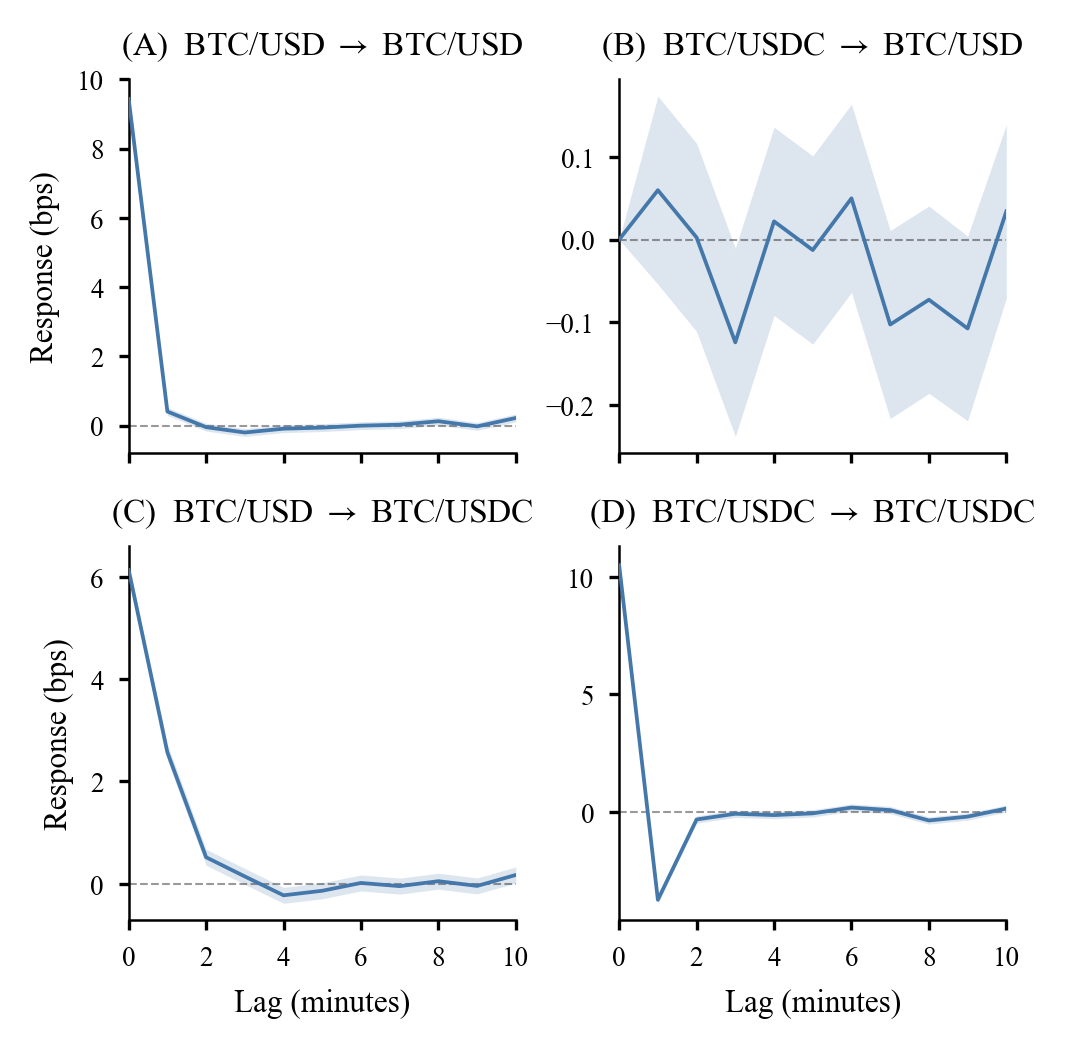
\includegraphics[width=\columnwidth]{figures_col/fig_var_irf.png}
    \caption{Orthogonalized IRF from VAR(10) on Kraken BTC/USD and BTC/USDC returns (bps). (B)~USDC$\to$USD: insignificant. (C)~USD$\to$USDC: significant (${\approx}6$ bps, decays in 3--4 min). Shaded: 95\% asymptotic CI.}
    \label{fig:irf}
\end{figure}

BH/FDR-corrected Granger tests on returns provide secondary evidence: BTC/USD $\to$ BTC/USDC is significant ($q<0.001$) but the reverse is not after FDR correction ($q=0.13$), consistent with fiat-to-stablecoin price adjustment. All other channels (USDT intra-exchange, cross-exchange) show bidirectional significance, consistent with active two-way arbitrage in more liquid markets.

\subsection{Arbitrage after fees}\label{sec:arb}
Having established that price discovery resides in the fiat-quoted channel, a natural question is whether the documented dislocations offer exploitable arbitrage opportunities. We evaluate this using explicit trade construction---3-leg triangular for intra-exchange stablecoin channels, 2-leg pre-funded buy/sell for cross-exchange---under two cost bounds:
\begin{align}
    \text{cost}^{\text{fee}}_t &= n_{\text{legs}}\cdot f, \\
    \text{cost}^{\text{fee+slip}}_t &= n_{\text{legs}}\cdot f + \sum_{\ell=1}^{n_{\text{legs}}}\tfrac{1}{2}\,\text{RangeProxy}_{\ell,t},
\end{align}
with $f=5$ bps per taker leg.

% Full-width figure (two panels)
\begin{figure}[H]
    \centering
    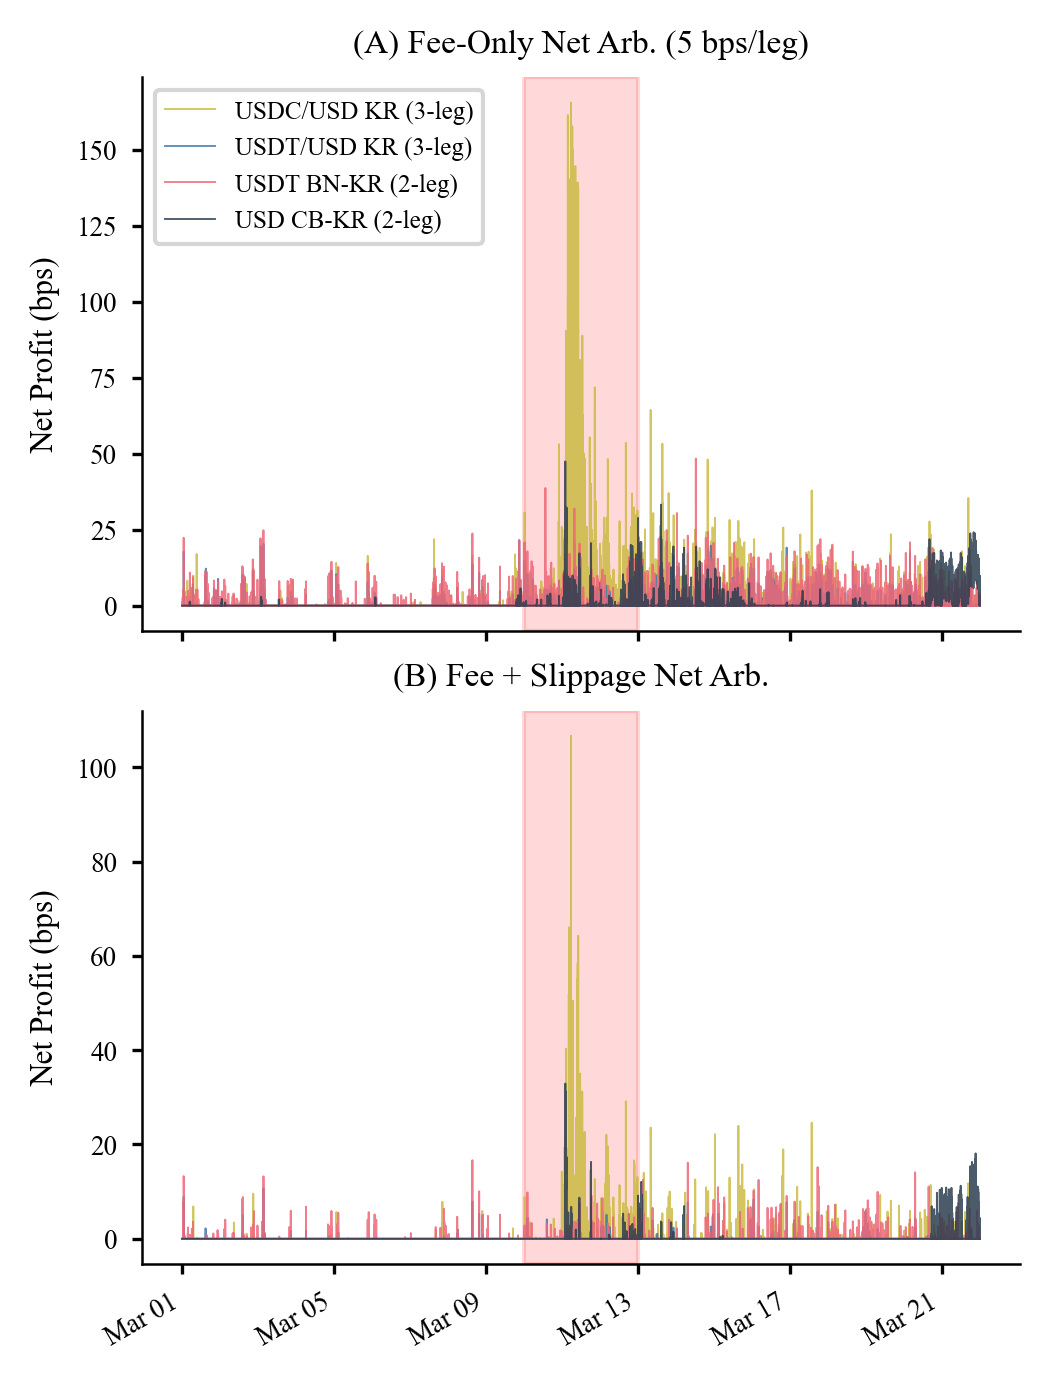
\includegraphics[width=\columnwidth]{figures_col/fig_arbitrage_after_fees.png}
    \caption{Net arbitrage profit (bps) under (A) fee-only costs (5 bps/leg) and (B) fee + range-based slippage. Crisis USDC profits compress sharply with slippage; cross-exchange profits are also attenuated.}
    \label{fig:arbfees}
\end{figure}


Figure~\ref{fig:arbfees} shows the time series of net arbitrage profits under both cost specifications. Adding range-based slippage (Panel~B) materially compresses profitability: USDC intra-exchange crisis profitability falls from $29.16\%$ to $6.72\%$ (net $4.83$ to $0.64$ bps); Coinbase--Kraken BTC/USD falls from $11.32\%$ to $2.29\%$. Fee sensitivity: at $f{=}3$ bps (maker rebate), USDC crisis fee+slippage profitability rises to $14.0\%$; at $f{=}10$ bps (retail), it falls to $1.0\%$. The narrow post-cost opportunities are consistent with limited executable arbitrage under realistic frictions.

\begin{table}[H]
\caption{Arbitrage profitability by channel/regime with 5 bps taker fees per leg (3-leg intra-exchange; 2-leg cross-exchange).}
\label{tab:arb}
\footnotesize
\resizebox{\columnwidth}{!}{%
\begin{tabular}{llcrr}
\toprule
Channel & Regime & Cost Variant & \%Profitable & AvgNetUncond (bps) \\
\midrule
USDC/USD (Kraken)      & Crisis   & Fee-only & 29.16 & 4.83 \\
USDC/USD (Kraken)      & Crisis   & Fee+slip &  6.72 & 0.64 \\
USDC/USD (Kraken)      & Post-SVB & Fee-only &  9.38 & 0.56 \\
USDC/USD (Kraken)      & Post-SVB & Fee+slip &  1.78 & 0.08 \\
USDT/USD (Kraken)      & Crisis   & Fee-only &  3.76 & 0.14 \\
USDT/USD (Kraken)      & Crisis   & Fee+slip &  0.37 & 0.01 \\
Cross BTC/USD (CB--KR) & Crisis   & Fee-only & 11.32 & 0.72 \\
Cross BTC/USD (CB--KR) & Crisis   & Fee+slip &  2.29 & 0.15 \\
Cross BTC/USDT (BN--KR)& Crisis   & Fee-only & 11.85 & 0.49 \\
Cross BTC/USDT (BN--KR)& Crisis   & Fee+slip &  1.81 & 0.05 \\
\bottomrule
\end{tabular}%
}
\end{table}

% ======================================================================
\section{Regulatory Interpretation}\label{sec:regulation}
% ======================================================================

The preceding analysis identifies a clear failure chain: reserve-access risk drives peg deviation, peg deviation drives dispersion---both mechanically through $D_t$ and via the contagion channel $\hat\lambda$ through $B_t$---and limited depth constrains arbitrage correction. We now ask whether the GENIUS Act's provisions target this chain. The results point to banking-layer reserve-access risk as the root cause. Circle held \$3.3B (${\approx}8\%$) of USDC reserves at SVB \cite{circle2023}; the ${\sim}940\times$ half-life gap (bootstrap $p{<}10^{-4}$) localizes persistent dislocation to the peg layer, and the significant $\hat\lambda$ confirms that this dislocation propagates beyond the mechanical channel. Sustained recovery required emergency deposit guarantees on March 16 \cite{jointstatement2023}.

The GENIUS Act (July 2025) targets four dimensions of this chain; we map provisions to results as consistency checks \cite{genius2025}. (i)~\emph{Reserve composition}: Table~\ref{tab:genius_cf} maps 25\%--75\% mitigation to implied $D_t$ of ${\approx}240$--$80$ bps. (ii)~\emph{Timely redemption}: the $572$-min peg half-life (vs.\ $1.06$ pre-SVB) quantifies the five-day redemption freeze. (iii)~\emph{Bankruptcy super-priority}: targets P99 tail risk ($81.4$ vs.\ $13.6$ bps). (iv)~\emph{Transparency}: traders learned of SVB exposure only from Circle's Friday-night disclosure, consistent with the USDC--USDT decorrelation ($\rho{=}0.16$).

\begin{table}[H]
\caption{Illustrative GENIUS Act scenario range (not causal): assumed mitigation of the reserve lock-up shock mapped to implied crisis $D_t$ means from observed moments. Tail benchmark: USDC crisis $B_t$ P99 = 81.4 bps vs.\ pre-crisis 13.6 bps.}
\label{tab:genius_cf}
\footnotesize
\resizebox{\columnwidth}{!}{%
\begin{tabular}{p{3.5cm}rrrp{4.8cm}}
\toprule
Scenario & Mitigation (\%) & Implied $D_t$ (bps) & Reduction (bps) & Policy mapping \\
\midrule
Observed baseline        &   0 & 320.0 &   0.0 & SVB/No GENIUS baseline \\
Low mitigation           &  25 & 240.0 &  80.0 & Reserve composition + redemption + transparency \\
Moderate mitigation      &  50 & 160.0 & 159.9 & Reserve composition + redemption + transparency \\
High mitigation          &  75 &  80.1 & 239.9 & Reserve composition + redemption + transparency \\
Full-mitigation lower bd & 100 &   0.1 & 319.9 & Reserve composition + redemption + transparency \\
\bottomrule
\end{tabular}%
}
\end{table}

Persistent cross-exchange deviations ($+2.18$ bps) and the $26\times$ depth gap suggest reserve-layer reforms alone may not eliminate spatial fragmentation.

% ======================================================================
\section{Conclusion}\label{sec:conclusion}
% ======================================================================

Four findings emerge. First, SVB-triggered fragmentation is attributable to stablecoin peg risk: $D_t$ reaches $+320$ bps but $B_t$ stays near $+5$ bps with sub-minute mean reversion; the ${\sim}940\times$ half-life gap is statistically confirmed (moving-block bootstrap 95\% CI $[216,\,1{,}898]$, $p{<}10^{-4}$), localizing persistent dislocation to reserve-access risk. Second, the contagion intensity model reveals that peg stress transmits to the adjusted basis beyond the mechanical channel: $\hat\lambda$ is significant during crisis ($p{<}0.001$) but not pre-SVB, with USDC and USDT transmitting in opposite directions consistent with de-peg versus safe-haven dynamics. Third, the crisis is USDC-specific: excess kurtosis $12.9$ ($6\times$ tail expansion), USDT safe-haven premium ($+58$ bps), and cross-stablecoin decorrelation ($0.44\to0.16$). Fourth, post-friction arbitrage narrows sharply ($29\%\to7\%$), with the $26\times$ depth gap limiting executable scale.

The GENIUS Act's provisions target precisely this failure chain. Because dislocation resides in the peg layer and propagates to the adjusted basis through the $\lambda$ channel, reforms reducing reserve-access risk should compress not only $D_t$ mechanically but also $B_t$ through the contagion pathway. However, persistent cross-exchange deviations and depth asymmetry suggest additional market-structure measures may also be needed. A natural next step is a post-GENIUS replication study during the next stress event.

\paragraph{Interpretation boundaries.} This evidence is window-specific (March~2023) and observational; $\hat\lambda$ measures Granger-predictive transmission, not structural causation. Policy passages are consistency mappings, not causal identification.
Robustness: (i)~HAC intervals preserve directional signs; (ii)~no-FF filters preserve rank-order conclusions; (iii)~$\hat\lambda$ is robust to no-FF and 5-minute sampling; (iv)~cointegration is rank-stable for BTC/USD--USDT but not USDC; (v)~Chow tests confirm the regime split.

\smallskip\noindent\textbf{Reproducibility.}
All exhibits are deterministic outputs of \texttt{run\_all.py}; artifact-label integrity is verified by \texttt{src/04\_tex\_integrity\_check.py}.

\small
\begin{thebibliography}{99}
\bibitem{amihud2002} Amihud, Y. (2002). Illiquidity and stock returns: Cross-section and time-series effects. \emph{Journal of Financial Markets}, 5(1), 31--56.
\bibitem{chow1960} Chow, G. C. (1960). Tests of equality between sets of coefficients in two linear regressions. \emph{Econometrica}, 28(3), 591--605.
\bibitem{circle2023} Circle (March 11, 2023). \emph{Silicon Valley Bank and USDC}. Circle update.
\bibitem{englegranger1987} Engle, R. F., \& Granger, C. W. J. (1987). Co-integration and error correction: Representation, estimation, and testing. \emph{Econometrica}, 55(2), 251--276.
\bibitem{jointstatement2023} Federal Reserve, FDIC, and U.S. Treasury (March 12, 2023). \emph{Joint statement by the Department of the Treasury, Federal Reserve, and FDIC}.
\bibitem{granger1969} Granger, C. W. J. (1969). Investigating causal relations by econometric models and cross-spectral methods. \emph{Econometrica}, 37(3), 424--438.
\bibitem{hasbrouck1995} Hasbrouck, J. (1995). One security, many markets: Determining the contributions to price discovery. \emph{Journal of Finance}, 50(4), 1175--1199.
\bibitem{johansen1988} Johansen, S. (1988). Statistical analysis of cointegration vectors. \emph{Journal of Economic Dynamics and Control}, 12(2--3), 231--254.
\bibitem{neweywest1987} Newey, W. K., \& West, K. D. (1987). A simple, positive semi-definite, heteroskedasticity and autocorrelation consistent covariance matrix. \emph{Econometrica}, 55(3), 703--708.
\bibitem{roll1984} Roll, R. (1984). A simple implicit measure of the effective bid-ask spread in an efficient market. \emph{Journal of Finance}, 39(4), 1127--1139.
\bibitem{genius2025} U.S. Congress (2025). \emph{Public Law 119-27: Guiding and Establishing National Innovation for U.S. Stablecoins Act (GENIUS Act)}.
\end{thebibliography}

\end{document}